%
% Name: Natural Language Processing
% Author: Donald Whyte (sc10dw@leeds.ac.uk)
%

\documentclass{article}

\usepackage[margin=2cm]{geometry} % easy page formatting
	\geometry{letterpaper}
\usepackage{doc} %special logo commands
\usepackage{url} % formatting URLs
\usepackage{datetime} % up-to-date, automatically generated times
% For graphic files
\usepackage{graphicx}
\usepackage{epstopdf}
\usepackage{float}
\usepackage{amsmath}
\DeclareGraphicsRule{.tif}{png}{.png}{`convert #1 `dirname #1`/`basename #1 .tif`.png}

% Set the title, author, and date.
\title{Natural Language Processing \\ COMP3310 -- AI32}
\author{Donald Whyte}
\date{\today}

% The document proper.
\begin{document}

% Add the title section.
\maketitle

% Add various lists on new pages.
\tableofcontents

\pagebreak
\listoffigures

\pagebreak
\listoftables

% Start the paper on a new page.
\pagebreak

\section{Words}

\subsection{Corpora}

A \textbf{corpus} is a finite body of naturally occurring text that is \textit{not} automatically generated or written specifically for use in NLP. The text used is normally selected according to criteria derived from the needs of the NLP application.

What corpus you use changes what you learn, so it is important to be careful and choose data representative of the problem you're trying to solve. For example, well-edited text (e.g. news articles) is better for deriving grammatical structure. Facebook conversations (say) would have a lot of incorrect spelling and grammar; these errors are simply noise that make it harder for AI to derive grammar.

Properties of corpora:
\begin{itemize}
	\item \textbf{Language Type} -- is it edit text, spontaneous speech? Is it written following standards or are there dialects present?
	\item \textbf{Genre and Domain} -- is it 18th century novels, newspaper text, train enquiry dialogue, FB conversations, etc.?
	\item \textbf{Media} -- text, audio or video?
	\item \textbf{Size} -- how large is the corpus. Bigger almost always means better!
\end{itemize}

A \textbf{balanced corpus} is one which tries to be representative across an entire language or domain. It contains many different tones of text from a language, instead of specifying a single area (not just news or FB conversations -- all kinds of text!)

Common corpora:
\begin{itemize}
	\item \textbf{Brown} -- Famous early corporate of 1 million words. Part-of-speech tagged. Balanced corpus of written American English.
	\item \textbf{LOB} -- Lancaster-Oslo/Bergen corpus. Published British English text.
	\item \textbf{Web 1T Corpus (2006)} -- 1 trillion words of text grabbed from the web, with many domains and languages.
	\item \textbf{Penn Treebank} -- \textbf{parsed}, not just tokenised, text of 2 million words. Domain is newswire and language is American English.
\end{itemize}

\subsection{Tokenisation}

\subsubsection{Definitions}

\textbf{Tokenisation} is a \textbf{processing step} where the input text is automatically divided into atomic units called tokens. A \textbf{token} is either a word, number, or a punctuation mark. \textbf{Word} throughout this document means:
\begin{quote}
	\textit{"continuous alphanumeric characters, delineated by whitespace"}
\end{quote}
where \textbf{whitespace} is spaces, tabs and newlines.

A token is an \textit{individual occurrence} of a word. A textbf{token type} is the word itself without context. For example, the sentence "what is the big elephant and what makes it big?" has 11 tokens (including the question mark) and 9 token types (what and big appear twice).

Delimiting by whitespace may not be enough however. Consider the case below:
Here "data base" carries the atomic meaning but will be considered \textit{two} tokens. Additionally, "it's," contains a \textit{trailing comma}. This is not desired because it makes it look like a different token type to "it's", so it may look like it has a different meaning (when it doesn't). Using \textbf{regular expressions} for tokenising may be more suitable, as it can deal with such cases (especially trailing punctuation).

\textbf{Lexical diversity} (see Equation) \ref{eq:lexical-diversity} measures how diverse the vocabulary of a body of a text is. This measurement is the \textbf{average} number of times a token type occurs in the text. Therefore, if the same words are used often there will be \textbf{high} lexical diversity. Likewise, if there is large variety of words, then lexical diversity will be \textbf{low}.

\begin{equation}
	\frac{numTokens}{numTokenTypes}
	\label{eq:lexical-diversity}
\end{equation}

\subsubsection{Issues}

\begin{itemize}
	\item \textbf{Sentence Boundaries} -- e.g. punctuation, quotation marks around sentences? What does a sentence begin/end? For example, "I said 'Bye Joe.' and laughed!". This a whole sentence, but a tokeniser might think "Joe." is the end of the sentence due to the full stop.
	\item \textbf{Proper Names} -- proper names are often composed of multiple words delimited by spaces, such as "Donald Whyte" or "New York". How do we detect that they belong together as a single unit?
	\item \textbf{Contractions/Possession} -- when is an apostrophe used for contractions or possession? "That’s Fred’s jacket’s pocket." should jacket's be expanded to "jacket is" just like that's to "that is"? What makes "jacket's" possession but not "that's"? How commonly it's usedas a contraction in labelled corpora?
\end{itemize}

\subsection{Morphology}

\textbf{Morphology} is the study of the way words are built up from \textbf{smaller meaning units}. \textbf{Morphemes} are the \textit{smallest meaningful unit} in the grammar of a language. A word is composed of one or more morphemes.

Morpheme definitions:
\begin{itemize}
	\item \textbf{Root} -- portion of word that is \textbf{common} to a set of derived or inflected forms when all \textbf{affixes are removed}. The root cannot be broken down into further analysable, meaning elements and it carries the \textbf{principle portion} of the meaning of the words.
	\item \textbf{Stem} -- The root(s) of a word with \textbf{derivational affixes} included, but \textbf{inflectional affixes removed} This form is ready for inflectional affixes to be added, but the stem does not contain these.
	\item \textbf{Affix} -- a \textbf{bound} morpheme that cannot be used by itself. It must be joined \textbf{before, after} or \textbf{within} a root or stem. There are four types of affixes:
	\begin{itemize}
		\item \textbf{Prefixes} -- before stem, such as \textbf{antidis}establishmentarianism
		\item \textbf{Suffixes} -- after stem, such as antidisestablish\textbf{mentarianism}
		\item \textbf{Infixes} -- in the middle of the stem. Hingi (borrow) to h\textbf{um}ingi (borrower) in Tagalog
		\item \textbf{Circumfixes} -- at the start and end of stem. Sagen(say) to \textbf{ge}sag\textbf{t} (said) in German
	\end{itemize}
	\item \textbf{Clitic} -- morpheme which functions \textbf{syntactically like a word}, but does not appear as an individual word
\end{itemize}

\textbf{"unladylike"} is a word with 3 morphemes and 4 syllables. The three morphemes are:
\begin{enumerate}
	\item "un-" -- means "not" (derivational affix)
	\item "lady" -- means "(well behaved) female adult human" (root)
	\item "-like" -- having the characters of (derivational affix)
\end{enumerate}
These three units cannot be broken down further \textit{without distorting the meaning of the units into something they're not}. The \textbf{stem} of "unladylike" is "unladylike" , since no inflectional affixes are used.

\textbf{"technique"} has a single morpheme and two syllables. The root and stem are therefore "technique" as well.

\textbf{"dogs"} has two morphemes and one syllable. The two morphemes are:
\begin{enumerate}
	\item "dog" -- animal (root)
	\item "-s" -- plural marker on nouns (inflectional)
\end{enumerate}
 The \textbf{stem} of "dogs" is "dog", as the inflectional affix "-s" has been removed.
 
\subsubsection{Inflectional}

\textbf{Inflection} is a variation in the form of a word that expresses a grammatical contrast. It doesn't change the word class but causes the word to serve a \textbf{new grammatical role}. Inflection adds tense, number/counts, person, mood and aspect to words.

The change is usually achieved by adding an \textbf{inflectional affix}. This affix usually produces a predictable change of meaning. That is, the change is consistent across most/all words. For example, "-s" is an inflection affix which typically pluralises nouns and makes transforms a verb:
\begin{quote}
	\textit{"apple -$>$ apples"}
\end{quote}
\begin{quote}
	\textit{"run -$>$ runs"}
\end{quote}

\subsubsection{Derivational}

\textbf{Derivation} is the formation of a new word or inflectable stem from another word or stem. An example of this is:
\begin{quote}
	\textit{"compute -$>$ computer -$>$ computerisation"}
\end{quote}
The two latter words contain the same root "compute", but through derivational affixes "-r" and "-isation" mean different things.

Derivation can \textbf{change the word class}, such as verb $\rightarrow$ noun and noun $\rightarrow$ adjective. For example, "compute" is a verb which is transformed into the noun "computer" by adding "-r".

\subsection{Stemming}

\textbf{Stemming} is the process of taking a word, complete with all its derivational and inflectional affixes and finding the \textbf{stem} of the original word. That is, a stemmer removes all inflectional affixes while leaving the stem intact.

Rule-based stemmers stem words based on rules. An example of this is the \textbf{Porter stemmmer}, which simply hacks off the end of the use. It is frequently used, especially for information retrieval, but the results are ugly.

Original:
\begin{quote}
Pierre Vinken , 61 years old , will join the board as a nonexecutive
director Nov. 29 . Mr. Vinken is chairman of Elsevier N.V. , the Dutch
publishing group . Rudolph Agnew , 55 years old and former chairman of
Consolidated Gold Fields PLC , was named a nonexecutive director of
this British industrial conglomerate . A form of asbestos once used to
make Kent cigarette filters has caused a high percentage of cancer
deaths among a group of workers exposed to it more than 30 years ago ,
researchers reported.
\end{quote}

Porter stemmed version:
\begin{quote}
Pierr Vinken , 61 year old , will join the board as a nonexecut
director Nov. 29 . Mr. Vinken is chairman of Elsevi N.V. , the Dutch
publish group . Rudolph Agnew , 55 year old and former chairman of
Consolid Gold Field PLC , wa name a nonexecut director of thi British
industri conglomer . A form of asbesto onc use to make Kent cigarett
filter ha caus a high percentag of cancer death among a group of
worker expos to it more than 30 year ago , research report .
\end{quote}

While the results are ugly, it might not matter. Bad stemming is not necessarily a problem for \textbf{automated information retrieval} as long as the stemming is \textit{consistently} bad/incorrect. If so, then the automated document searching, which is based on keywords that also get stemmed using the same stemmer, will still work efficiently, taking into consideration correct word stems (correct in that they are consistently incorrect).

WordNet's morphy() is a slightly more sophisticated rule-based stemmer. It uses different rules based on the part-of-speech tag of a word and has an exception list for irregular words. Some of the rules are listed in Figure\ref{fig:morphy-rules}

\begin{figure}
	\centering
	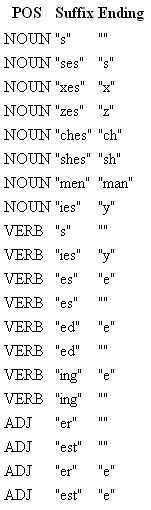
\includegraphics[scale=0.4]{figures/morphy-rules.png}
	\caption{Portion of Rules the Stemmer Morphy Uses}
	\label{fig:morphy-rules}
\end{figure}

One approach is to "cheat" and not use rules at all. Instead, all variants of a stem are stored in a \textbf{dictionary}. Stepping a word is simply a matter of looking up that word in a dictionary and retrieving the associated stem.

\textbf{Categorical Variation Database (CatVar)} is a "database of clusters of uninflected words and their categorical (i.e. part-of-speech) variants".

Rule-based systems and dicitonary systems cannot \textbf{generalise} to different languages. \textbf{Unsupervised Machine learning}, on the other hand, can be used to find recurring patterns in languages which researchers can use to understand how to stem words in any language better.

\section{Counting Words}

\subsection{Frequency Distributions}

\textbf{Word frequency} is the number of types a token type appears in the text. \textbf{Absolute frequency} is the number of times a word occurs in a body of text. \textbf{Relative frequency} is the number of times a word occurs in a body of text, \textbf{relative} to all the other words in the text (i.e. the text's size). Relative frequency is computed using Equation \ref{eq:rel-freq}, where $f(x)$ is the frequency of word $x$ and $T$ is a list of all the tokens/words in the document.

\begin{equation}
	rf(x) = \frac{frequency\;of\;x}{total\;frequency} =
	\frac{f(x)}{ \sum_{y \in T} {f(y)} }
	\label{eq:rel-freq}
\end{equation}

The frequencies of all word \textit{types} can be counted and put in a \textbf{frequency distribution}, which is table of word types and their frequencies (\textbf{ordered} from most frequency to least). Table \ref{tab:freqdist} and Figure \ref{fig:freqdist} shows an examples of frequency distribution tables and plots.

\begin{table}
	\centering
	\begin{tabular}{|l|l|}
		\hline
		\textbf{Token} & \textbf{Frequency} \\
		\hline
		the & 350 \\
		and & 212 \\
		to & 191 \\
		of & 167 \\
		a & 165 \\
		i & 160 \\
		that & 134 \\
		... & ...\\
		but & 68 \\
		... & ...\\
		donald & 1 \\
		\hline
	\end{tabular}
	\caption{Example Frequency Distribution Table (ordered from most-frequent to least)}
	\label{tab:freqdist}
\end{table}

\begin{figure}
	\centering
	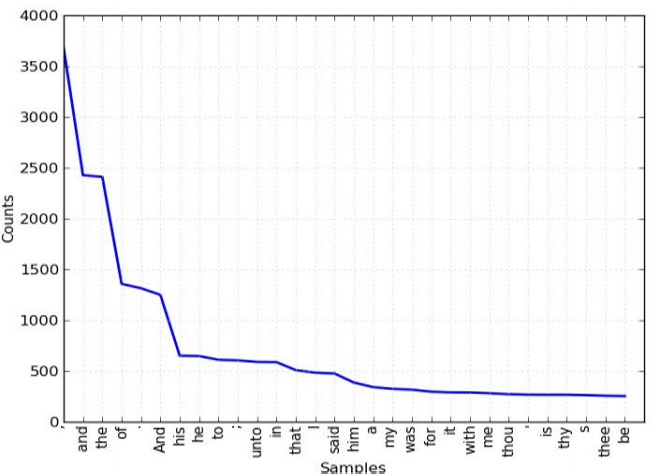
\includegraphics[scale=0.4]{figures/frequency-distribution.png}
	\caption{Example Frequency Distribution Table (ordered from most-frequent to least)}
	\label{fig:freqdist}
\end{figure}

\subsection{Zipf's Law}

The \textbf{rank} of a word is its position in an ordered frequency distribution table. If a word has a rank of 1, it is the \textbf{most frequent} word in the text.

\textbf{Zipf's law} captures the relation between the frequency and rank of a word. Let $r$ and $f$ be the rank and frequency of a word. There is a constant $k$ such that:
\begin{equation}
	k = f \cdot r
\end{equation}
Alternative, $f$ is proportional to $r$ like so:
\begin{equation}
	f \propto \frac{1}{r}
\end{equation}

The plot on the right of Figure \ref{fig:zipf} is a logarithmic plot that this relation, as the plot is roughly a straight line. Figure \ref{fig:zipf-corpus} plots the frequency distribution of a one million word corpus (rank/freq, not word itself) against Zipf's law. As evident by these plots, Zipf's law does apply to real, natural text.

\begin{figure}
	\centering
	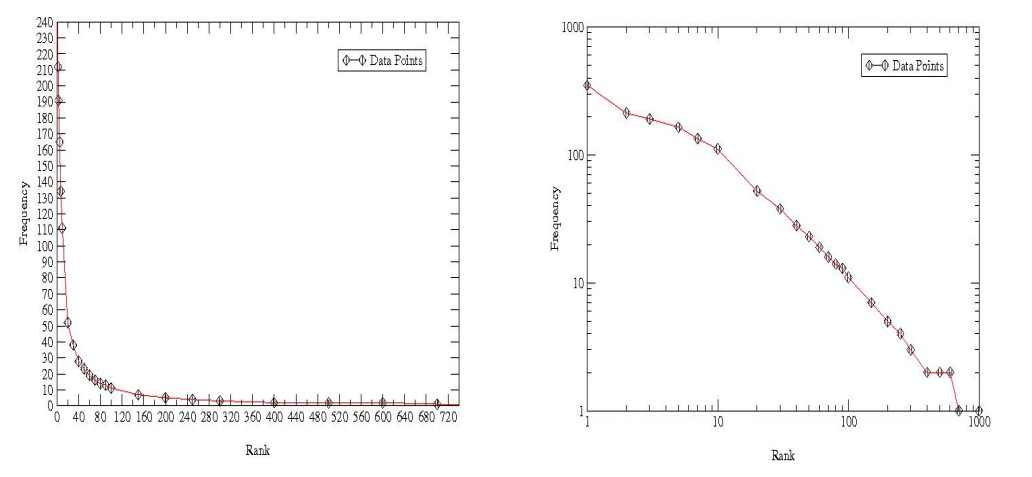
\includegraphics[scale=0.4]{figures/zipfs-law.png}
	\caption{Zipf's Law: Plots of rank against frequency, shows exponential relationship. With logarithmic plot, relationship is linear.}
	\label{fig:zipf}
\end{figure}

\begin{figure}
	\centering
	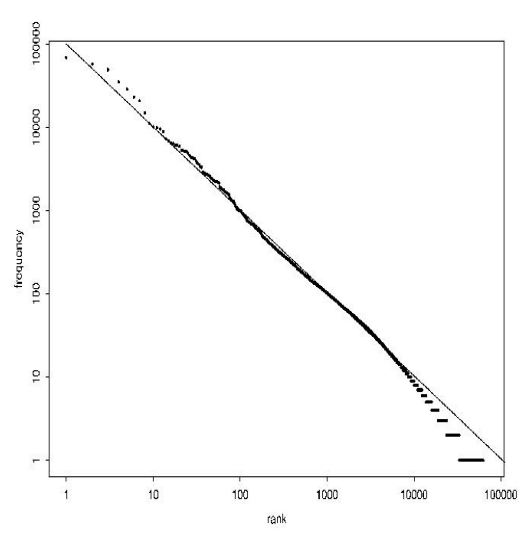
\includegraphics[scale=0.4]{figures/brown-zipfs-law.png}
	\caption{Brown Corpus Logarithmic Plot Against Zipf's Law}
	\label{fig:zipf-corpus}
\end{figure}

So what does this mean?
\begin{itemize}
	\item There is a \textbf{very small number of very common words}
	\item There is a small-medium number of middle frequency words
	\item There is a \textbf{very large number of words which are infrequent} (especially words with a frequency of one)
	\item The relationship between frequency and rank can be \textbf{approximated by a line} (in logarithmic scales)
	\item This is different from the bell curve/normal distribution (which is a common statistical distribution for real word data)
\end{itemize}

Zipf's law highlights a common issue that affects many NLP techniques. \textbf{Data sparseness} refers to the fact that most words will have very few, or no, examples in training data. This leads to unreliable frequency counts and probabilities, which are often used in NLP.

\section{Information Retrieval}

\subsection{Definition}

Information retrieval (IR) addresses the following task:
\begin{quote}
	given a query, find documents that are "relevant" to the query
\end{quote}

The problem has the following inputs and outputs:
\paragraph{} \begin{tabular}{ll}
	\textbf{Input:} & a large, static document collection \\
	\textbf{Input:} & keyboard-based query \\
	\textbf{Output:} & find all documents relevant to query, and \textbf{only} those relevant documents \\
\end{tabular}

A \textbf{document} here refers to a body of text, but IR extends beyond items of text -- it can be any item you want to find (e.g. image, video, etc.) A document is described by a set of \textbf{index terms}, which in this case are the words in the document. 

\paragraph{}

Example uses of IR systems include:
\begin{itemize}
	\item search set of abstracts (of research papers)
	\item search newspaper article
	\item library search
	\item search the web
\end{itemize}

\subsection{Architecture}

Figure \ref{fig:ir-architecture} shows the architecture of a typical IR system. IR systems have \textbf{three main components}:
\begin{itemize}
	\item \textbf{Query Matcher} -- matches a given query to set of documents it believes are relevant to said query
	\item \textbf{Learning Component} -- receives feedback from the user and from that the system learns about which documents are relevant to which queries/terms
	\item \textbf{Object Base} -- database of documents and their index terms (descriptions)
\end{itemize}

An example sequence of events is:
\begin{enumerate}
	\item \textbf{User} enters query "red trousers"
	\item \textbf{Query Matcher} uses that to find three documents in the \textbf{Object Base} it believes are relevant to "red trousers" and returns them to the user
	\item \textbf{User} gives feedback about which of the three documents were relevant or not (e.g. clicking on web page, explicitly clicking "not relevant" button", etc.)
	\item \textbf{Learning Component} uses this feedback to learn/alter itself to reduce the chances of the documents marked irrelevant show up the next time someone types "red trousers". This may involve updating documents' descriptions in the \textbf{Object Base}.
\end{enumerate}

\begin{figure}
	\centering
	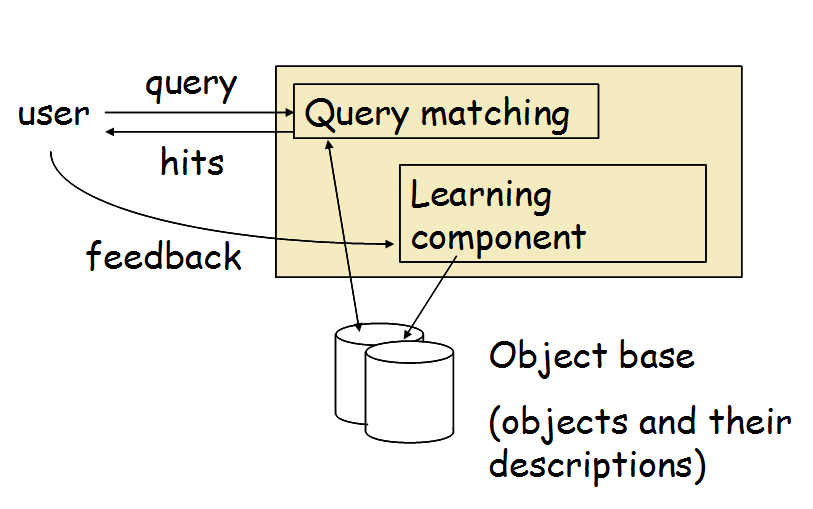
\includegraphics[scale=0.4]{figures/ir-system-architecture.png}
	\caption{Architecture of Information Retrieval Systems}
	\label{fig:ir-architecture}
\end{figure}

\subsection{Indexing}

Automatic indexing is a process which associates documents to index terms (descriptors) for fast look-up by the query matcher. If we consider \textbf{documents} to be bodies of text and the words contained with the text to be the \textbf{index terms}, then an \textbf{inverted file structure} can be established.

First we construct a list of numbered documents and the words contained within each document, as shown in Table \ref{tab:doc-word}. This may involve removing case (e.g. all lowercase), punctuation and common words, such as "the" and "at", which have little semantic meaning (known as \textbf{stopwords}) so only meaningful tokens remain. We could even stem words or use pairs of words (bigrams, computationally expensive) for collocation information.

We then \textbf{invert} the table so it is indexed by words, instead of documents. This creates a list of words and the documents those words are present in, like the one in Table \ref{tab:word-doc}.

More sophisticated inverted file structures can be created, which can track the \textbf{frequency} of a word in a document and its \textbf{position} in the document. Table\ref{tab:word-doc-sophisticated} shows an inverted file structure which lists the \textit{index} position of the token in the document (e.g. 'cold' is the 6th word in document 1).

\begin{table}
	\centering
	\begin{tabular}{|l|l|}
		\hline
		\textbf{Document} & \textbf{Text} \\
		\hline		
		1 & Pease porridge hot, pease porridge cold \\
		2 & Pease porridge in the pot \\
		3 & Nine days old \\
		4 & Some like it hot, some like it cold \\
		5 & Some like it in the pot \\
		6 & Nine days old \\
		\hline				
	\end{tabular}
	\caption{List of documents and the tokens contained within those documents}
	\label{tab:doc-word}
\end{table}

\begin{table}
	\centering
	\begin{tabular}{|l|l|l|}
		\hline
		\textbf{Number} & \textbf{Tokens} & \textbf{Documents} \\
		\hline
		1 & cold & 1,4 \\
		2 & days & 3,6 \\
		3 & hot & 1,4 \\
		4 & in & 2,5 \\
		5 & it & 4,5 \\
		6 & like & 4,5 \\
		7 & nine & 3,6 \\
		8 & old & 3,6 \\
		9 & pease & 1,2 \\
		10 & porridge & 1,2 \\		
		11 & pot & 2,5 \\
		12 & some & 4,5 \\
		13 & the & 2,5 \\		
		\hline
	\end{tabular}
	\caption{List of tokens and the documents those tokens are contained in}
	\label{tab:word-doc}
\end{table}

\begin{table}
	\centering
	\begin{tabular}{|l|l|l|}
		\hline
		\textbf{Number} & \textbf{Tokens} & \textbf{(Document; Word Index)} \\
		\hline		
		1 & cold & (1;6), (4;8) \\
		2 & days & (3;2), (6;2) \\
		3 & hot & (1;3), (4;4) \\
		4 & in & (2;3), (5;4) \\
		5 & it & (4;3,7), (5;3) \\
		6 & like & (4;2,6), (5;2) \\
		7 & nine & (3;1), (6;1) \\
		8 & old & (3;3), (6;3) \\
		9 & pease & (1;1,4), (2;1) \\
		10 & porridge & (1;2,5), (2;2) \\		
		11 & pot & (2;5), (5;6) \\
		12 & some & (4;1,5), (5;1) \\
		13 & the & (2;4), (5;5) \\	
		\hline
	\end{tabular}
	\caption{List of tokens and the documents those tokens are contained in (augmented with the \textbf{location} of the token in the document(s))}
	\label{tab:word-doc-sophisticated}
\end{table}

\begin{figure}
	\centering
	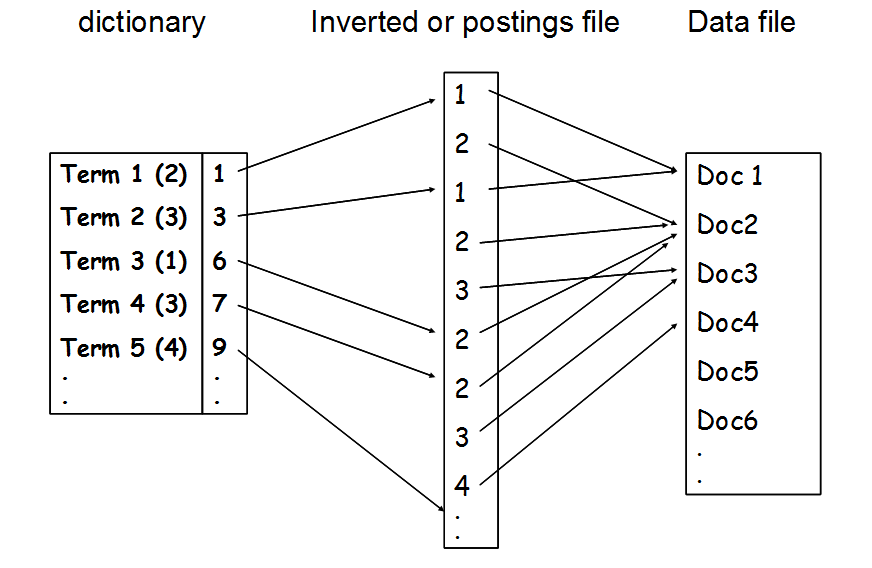
\includegraphics[scale=0.4]{figures/inverted-file-structure.png}
	\caption{Inverted File Structure}
	\label{fig:inverted-file-structure}
\end{figure}

Indexing as many documents as possible sounds like a good way to provide a \textbf{more comprehensive search}, but it may not be the thing to do.  There are \textbf{disadvantages}:
\begin{itemize}
	\item if you only want to look at a certain type of document, it is much more difficult to get precise, relevant hits when everything but the kitchen sink is in the system
	\item more documents means greater storage requirements and slower processing/search times
	\item more documents might not always given you \textit{new} information. You could have five different documents which all contain the same information -- why have all three?
\end{itemize}

\subsection{Notation}

We now deal with the \textbf{Query Matcher} component of the IR system. That is, how do we find documents relevant to a given a \textbf{search query}?

\paragraph{}

\begin{tabular}{p{4cm}p{12cm}}
	$D$ & list of $m$ documents \\
	$m$ & number of documents \\
	$T$ & list of index terms (words) \\
	$n$ & number of index terms \\
	$w_{ij}$ & \textbf{weight of association} between the $i$th index term $i$ and the $j$th document \\
	$d_j = (w_{1,j}, w_{2,j}, ..., w_{i,j})$ & Index term vector for $j$th document, which contains the weights between all index terms and document $j$.
\end{tabular}

\paragraph{}

\begin{tabular}{p{16cm}}
	\textbf{Example} \\
	$T = \lbrace pudding, jam, traffic, lane, treacle \rbrace$ \\
	$d_1 = (1, 1, 0, 0, 0)$ \\
	$d_2 = (0, 0, 1, 1, 0)$ \\
	$d_3 = (1, 1, 1, 1, 0)$ \\
\end{tabular}

\subsection{Set Theoretic Model}

The \textbf{set theoretic} model uses set theory to find documents which uses \textbf{boolean expressions} as search queries, like the one in Equation \ref{eq:set-theoretic-query}. After receiving such a query, the following steps are performed:
\begin{enumerate}
	\item the query is transformed into \textbf{Disjunctive Normal Form (DNF)} (example in Equation \ref{eq:set-theoretic-dnf})
	\item let $R = \emptyset$ be the set containing
	\item for each document $d_j = (w_{1,j}, w_{2,j}, ..., w_{i,j})$:
	\begin{enumerate}
		\item take the truth values (weights) in $d_j$ and check if it matches \textit{any} component of the DNF equation. This process is denoted using Equation \ref{eq:set-theoretic-similarity}
		\item if the output of the DNF expression was 1, then the document matches the original boolean query exactly. Add $d_j$ to $R$
	\end{enumerate}
	\item return $R$
\end{enumerate}

\begin{equation}
	(Jam \lor Treacle) \land Pudding \land \neg{Lane} \land \neg{Traffic}
	\label{eq:set-theoretic-query}
\end{equation}

\begin{equation}
	(1, 1, 0, 0, 0) \lor (1, 0, 0, 0, 1) \lor (1, 1, 0, 0, 1)
	\label{eq:set-theoretic-dnf}
\end{equation}

\begin{equation}
	sim(d, q_{DNF}) = \begin{cases}
		1,& \text{if }d\text{ is equal to any component of }q_{DNF} \\
		0,& \text{otherwise}
	\end{cases}
	\label{eq:set-theoretic-similarity}
\end{equation}

\paragraph{\textbf{EXAMPLE}} Taking the three documents $d_1$, $d_2$ and $d_3$, as well as the query and its DNF equivalent in Equations \ref{eq:set-theoretic-query} and \ref{eq:set-theoretic-dnf}, an example of using the set theoremtic model to find which documents are relevant to the query is given. Steps:
\begin{enumerate}
	\item Does $d_1 = (1, 1, 0, 0, 0)$ match a component in the DNF equation? \textbf{Yes}, $R = R \cup \lbrace d_1 \rbrace$.
	\item Does $d_2 = (0, 0, 1, 1, 0)$ match a component in the DNF equation? \textbf{No}, don't add $d_2$ to $R$.
	\item Does $d_3 = (1, 1, 1, 1, 0)$ match a component in the DNF equation? \textbf{No}, don't add $d_3$ to $R$.
\end{enumerate}
$R =  \lbrace d_1 \rbrace$, so only one relevant document is returned ($d_1$).

\begin{figure}[H]
	\centering
	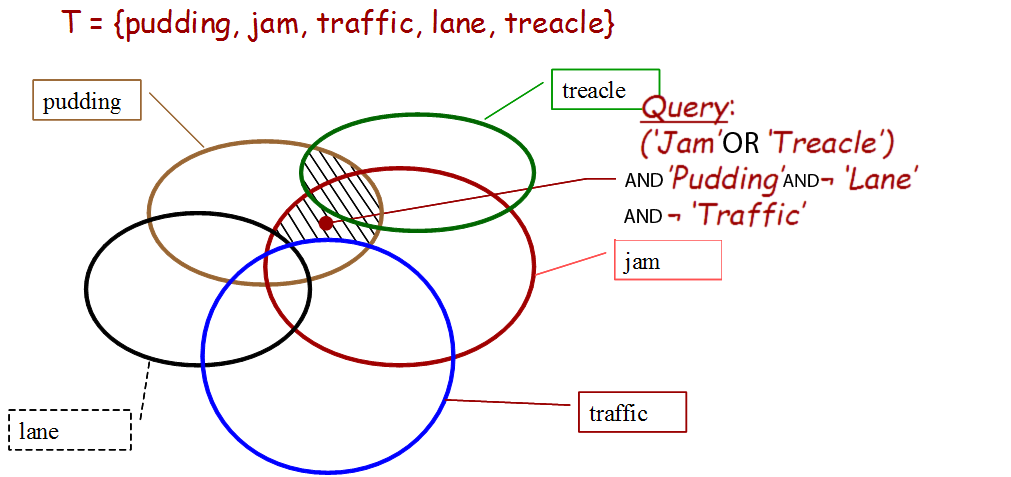
\includegraphics[scale=0.3]{figures/ir-set-theoric-venn1.png}
	\caption{Venn Diagram Illustrating what a Set Theoretic Search Query Does}
	\label{fig:ir-set-theoric-venn1}
\end{figure}

\begin{figure}[H]
	\centering
	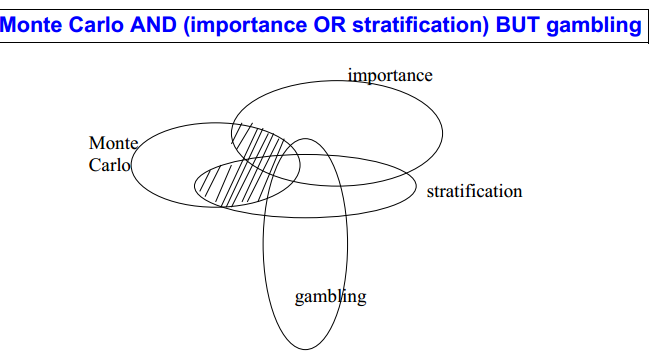
\includegraphics[scale=0.4]{figures/ir-set-theoric-venn2.png}
	\caption{Venn Diagram Illustrating what a Set Theoretic Search Query Does}
	\label{fig:ir-set-theoric-venn2}
\end{figure}

\subsubsection{Summary}

\paragraph{\textbf{Advantages}}
\begin{itemize}
	\item Boolean model is simple and queries have \textbf{precise semantics}, giving user complete control
	\item Popular with bibliographic systems and also available on some search engines
	\item Set-theoretic model can be extended to form a partial-matching system using \textbf{Fuzzy set model} and the \textbf{extended Boolean model}
\end{itemize}
\paragraph{\textbf{Disadvantages}}
\begin{itemize}
	\item Only returns \textbf{exact matches}. What if the user didn't know exactly what they were looking for or how to phrase it?
	\item Users find boolean queries hard to formulate
\end{itemize}

\subsection{Vector Space Model}

The \textbf{vector space model} treats documents as points in \textbf{high dimensional space}. Queries are also represented in vector space. Documents with the highest document-query similarity are selected. An \textbf{ordered list of relevant documents} is returned, going from \textbf{most relevant to least} (based on the similarity measure used).

Figure \ref{fig:vector-space-model} shows an IR system with three documents and two index terms, "car" and "insurance". The three documents and the given input query are represented as vectors in the space of index terms (which is 2D in this case as there are two terms). $d_3 = (5, 1)$ because it has 5 occurrences of insurance and 1 occurrence of car. This means that the \textbf{document-term weights are no longer binary values}.

Therefore, an $m \times n$ \textbf{document-by-word} matrix $M$ is constructed, where the rows are documents, the columns are terms and entry $M_{ij}$ is the \textbf{frequency} of the $j$th term appearing in the $i$th document. A query is a \textbf{vector} $q$ of size $n$, which contains weightings for each index term. An example of these is shown in Tables \ref{tab:doc-by-word-vector-space} and \ref{tab:query-vector-space}.

\begin{table}[H]
	\centering
	\begin{tabular}{|p{1cm}|p{1cm}p{1cm}p{1cm}p{1cm}p{1cm}|}
	\hline
	& $Term_1$ & $Term_2$ & $Term_3$ & ... & $Term_n$ \\
	\hline
	$Doc_1$ & 14 & 6 & 1 & ... & 0 \\
	$Doc_2$ & 0 & 1 & 3 & ... & 1 \\
	$Doc_3$ & 0 & 1 & 0 & ... & 2 \\
	... & ... & ... & ... & ... & ... \\
	$Doc_n$ & 4 & 7 & 0 & ... & 5 \\
	\hline
	\end{tabular}
	\caption{Example Document-By-Word Matrix with Word Frequencies}
	\label{tab:doc-by-word-vector-space}
\end{table}

\begin{table}[H]
	\centering
	\begin{tabular}{|p{1cm}|p{1cm}p{1cm}p{1cm}p{1cm}p{1cm}|}
	\hline
	$q$ & 0 & 1 & 0 & ... & 1 \\
	\hline
	\end{tabular}
	\caption{Example Query Vector with Weightings for each Index Term}
	\label{tab:query-vector-space}
\end{table}

\subsubsection{Similarity Measure}

A \textbf{similarity measure} $sim(\vec{d}, \vec{q})$, which compares the similarity between a document $\vec{d}$ and a search query $\vec{q}$ must be given. The similarity measure uses throughout this module summary is in Equation \ref{eq:cosine-similarity}. This is the \textbf{cosine} of the two vectors and measures the angle between two vectors in vector space. \textbf{Smaller angles} between the documents mean they are more similar and the opposite for larger angles. This also \textbf{normalises} the output so long documents don't \textbf{skew the ranked list} of relevant documents with larger values.

\begin{equation}
	sim(\vec{d}, \vec{q}) = cos(\vec{d}, \vec{q}) = \frac{\vec{d} \cdot \vec{q}}{|\vec{d}| |\vec{q}|}
	\label{eq:cosine-similarity}
\end{equation}

Figure \ref{fig:cosine-similarity} illustrates how this similarity measure \textbf{relates to} the spatial representation of the documents and query. Let $\vec{d_1}$ and $\vec{d_2}$ be two documents and $\vec{q}$ be a query. The angles between vectors $\vec{d_1},\vec{q}$ and $\vec{d_2},\vec{q}$ are measured. Whichever vector has the \textbf{smaller angle} is more similar to the query and is thus, a \textbf{better match}. In Figure \ref{fig:cosine-similarity}, it appears as if the angle between $\vec{d_1},\vec{q}$ is smaller, therefore $\vec{d_1}$ is a better match to the query $\vec{q}$ than $\vec{d_2}$.

Table \ref{tab:cosine-similarity-example} and Equation \ref{eq:cosine-similarity-example} show the cosine similarity function applied to two documents, given a query $q$.

\begin{figure}
	\centering
	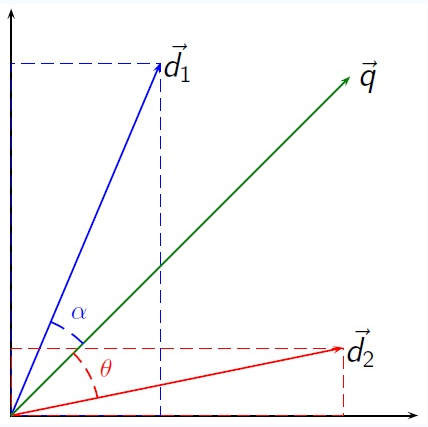
\includegraphics[scale=0.3]{figures/cosine-similarity.png}
	\caption{Cosine Similarity of Vectors}
	\label{fig:cosine-similarity}
\end{figure}

\begin{table}[H]
	\centering
	\begin{tabular}{|r|l|l|l|}
		\hline
		& $q$ & $d_{7655}$ & $d_{454}$ \\
		\hline
		hunter & 19.2 & 56.4 & 112.2 \\
		gatherer & 34.5 & 122.4 & 0 \\
		Scandinavia & 13.9 & 0 & 30.9 \\
		30,000 & 0 & 457.2 & 0 \\
		years & 0 & 12.4 & 0 \\
		BC & 0 & 200.2 & 0 \\
		prehistoric & 0 & 45.3 & 0 \\
		deer & 0 & 0 & 23.6 \\
		rifle & 0 & 0 & 452.2 \\
		Mesolithic & 0 & 344.2 & 0 \\
		\hline
	\end{tabular}
	\caption{Two documents and a query vector represented in 10D term space, with weights for each 10 terms}
	\label{tab:cosine-similarity-example}
\end{table}

\begin{multline}\\
	sim(d_{7655}, q) = cos(d_{7655}, q) = \frac{d_{7655} \cdot q}{|d_{7655}| |q|} = \frac{5305.68}{41.86(622.86)} = \frac{5305.68}{26071.72} = 0.20 \\
	sim(d_{4655}, q) = cos(d_{454}, q) = \frac{d_{454} \cdot q}{|d_{454}| |q|} = \frac{2583.75}{41.86(467.53)} = \frac{2583.75}{19569.97} = 0.13 \\
	cos^{-1}(0.20) = 78.46^{\circ}
	\;\;\;\;\;\;\;\;\;\;\;
	cos^{-1}(0.13) = 82.53^{\circ} \\
	\label{eq:cosine-similarity-example}
\end{multline}

\subsubsection{Term Weighting}

So how do we decide what \textbf{weights} to given each index term in the documents and in the search query $q$? We could use the \textbf{frequency} of the term in documents, but what if the term is generally frequent in \textbf{all documents}? Then, it doesn't really you find relevant documents, as all documents contain the word. This highlights a key issue:
\begin{quote}
	\textbf{Not all terms describe a document equally well!}
\end{quote}

\paragraph{}

\begin{tabular}{ll}
	\textbf{Definitions} & \\
	$tf_{w,d}$ & number of times word $w$ occurs in document $d$ \\
	$df_w$ & number of documents that contain $w$ \\
	$|D|$ & total number of documents in IR system 
\end{tabular}

Terms which are \textbf{frequent in a document} are better: $tf_{w,d} = freq_{w,d}$. Terms that are \textbf{rare in the overall document} collection are better: $idf_{w,D} = \log_{10} \frac{|D|}{df_w}$. Therefore, we combine these two measurements using Equation \ref{eq:tf-idf} to formulate a measurement of how \textbf{useful a term is at describing  a specific document}. This measurement is called \textbf{TF/IDF}.

\begin{equation}
	tfidf_{w,d,D} = tf_{w,d} \cdot idf_{w,D} = freq_{w,d} \cdot \log_{10} \frac{|D|}{df_w}
	\label{eq:tf-idf}
\end{equation}

This combined measurement gives high weighting to frequent terms, but \textbf{penalises} terms which are frequent in \textit{all} documents, as they are less helpful in distinguishing which documents are relevant and which are not).

Table \ref{tab:tf-idf} lists some terms and their frequency within a document $d$ and the whole document collection $D$. It also contains the TF/IDF measurement for each word. Notice how "general" has low frequency compared to "the", but since it appears in much less documents in the overall collection, it has a much higher weighting when using TF/IDF. The process of computing the TF/IDF value for the word "the" is shown in Equation \ref{eq:tf-idf-example}.

\begin{table}[H]
	\centering
	\begin{tabular}{|l|l|l|l|l|}
		\hline
		\textbf{Term} & $tf_{w,d}$ & $df_w$ & $|D|$ & TF/IDF ($tfidf_{w,d,D}$) \\
		\hline
		the & 312 & 28,799 & 30,000 & 500 \\
		in & 179 & 26,452 & 30,000 & 9.78 \\
		general & 136 & 179 & 30,000 & 302.50 \\
		fact & 131 & 231 & 30,000 & 276.87 \\
		explosives & 63 & 98 & 30,000 & 156.561 \\
		nations & 45 & 142 & 30,000 & 104.62 \\
		haven & 37 & 227 & 30,000 & 78.48 \\
		\hline
	\end{tabular}
	\caption{Table showing frequencies of words for a specific document $d$ for a collection of documents $D$. The TF/IDF index of each word for document $D$ is given.}
	\label{tab:tf-idf}
\end{table}

\begin{multline}\\
	idf_{the,D} = \log_{10} \frac{30,000}{28,799} = 0.0178 \\
	tf_{the,d} = freq_{w,d} = 312 \\
	tfidf_{the,d,D} = tf_{the,d} \cdot idf_{the,D} = 312 \cdot 0.0178 = 5.55 \\
	\label{eq:tf-idf-example}
\end{multline}

\subsubsection{Summary}

\paragraph{\textbf{Advantages}}
\begin{itemize}
	\item The vector space model is simply, \textbf{fast} and leads to "good" results
	\item \textbf{Partial matching} makes it more likely the user will get a hit, and also allows for ranked list of outputted documents
	\item Popular model for search engines
\end{itemize}
\paragraph{\textbf{Disadvantages}}
\begin{itemize}
	\item Makes the assumption that terms are \textbf{independant}. This is \textbf{not realistic}, as natural language has phrases, collocations and grammar.
\end{itemize}

\subsection{Manipulation of IR Systems}

One big limitation with IR systems is that they're often \textbf{easy to manipulate}. Many people exploit web search engines to get their pages high in searches, for example. One might hide loads of terms in their web pages which fool IR systems in thinking the page is relevant when it's not (causing the user to visit it). This is why most systems' query ranks are \textbf{supplemented by popularity measures} (e.g. page hits), so that kind of abuse is prevented.

\subsection{IR vs. Databases}

So what stops us from simply using a \textbf{DBMS (Database Management System)} to store documents and just using database queries to find what we want? Depending on the system and use case, it may actually make sense to do that instead. Table \ref{tab:ir-db-comparison} compares the two different approaches. The core difference is that DBMSes require exact queries to be inputted and output exact matches. IR systems are less sensitive to variance, requiring a loose query from the user and outputs \textit{likely} matches.
 
\begin{table}
	\centering
	\begin{tabular}{|l|l|l|}
		\hline
		& \textbf{DBMS} & \textbf{IR} \\
		\hline
		\textbf{match} & exact & partial or best match \\
		\textbf{inference} & deduction & induction \\
		\textbf{model} & record/field & text document \\
		\textbf{query language} & artificial & natural? \\
		\textbf{query specification} & complete & incomplete \\
		\textbf{items wanted} & matching & relevant \\
		\textbf{error response} & sensitive & insensitive \\
		\hline
	\end{tabular}
	\caption{Comparison of Information Retrieval to DBMS for Document Searching}
	\label{tab:ir-db-comparison}
\end{table}

\subsection{Query Broadening}

\begin{quote}
	\textbf{CURRENTLY NOT GOING TO FILL IN THIS ENTIRE SUB-SECTION!!!}
\end{quote}

TODO: main idea???

\subsubsection{Relevance Feedback}

TODO: formulae

TODO: example

TODO: PROS/CONS

todo: positive and negative feedback

\subsubsection{Thesaurus/Ontology}

TODO: definition

TODO: synonyms, hypernyms, hyponyms

TODO: coordinate terms

\subsubsection{Language Normalisation}

TODO: what this is with architecture

TODO: example

TODO: how it uses ontology (thesaurus use)

\section{Text Classification}

Text classification can be thought as a \textbf{standing query}, which is when you run a query periodically to find \textbf{new} items. The query does not rank items but \textbf{classifies} them as relevant vs. not relevant (to a specific topic). This section will focus on \textbf{topic classification}. An example of topic classification isdetermining if an email is spam or not, or what topic a news article is about (e.g. technology, economics, biology, etc.).

\paragraph{}

\begin{tabular}{ll}
\textbf{Problem Definition} \\
\textbf{Given} & a representation of a \textbf{document} $d$ \\
& a fixed set of \textbf{classes} (or labels or categories) $C = \lbrace c_1, c_2, ..., c_j \rbrace$ \\
\textbf{Determine} & \textbf{category} of $d$, $\gamma(d) \in C$ \\
& where $\gamma$ is a \textbf{classification function} that maps documents onto classes \\
\end{tabular}

\subsection{Classification Methods}

Documents can be \textbf{manually} by humans. This typically results in higher accuracy, but is much, much slower. \textbf{Hand-coded rule-based} classifiers are also possible, but to correctly classify even the simplest of documents, very precise rules are required. The rules must constantly evolve to handle outliers/corner cases that are always found. It's very hard to do in the long term.

Another approach is to use \textbf{supervised machine learning}, which produces a classification function based on \textbf{training dataset}. This is described more in Section \ref{sec:bow-text-classification}.

\subsection{BOW Text Classification}
\label{sec:bow-text-classification}

\begin{tabular}{p{7cm}p{10cm}}
\textbf{Supervised Machine Learning} \\
\textbf{Definition} \\
\textbf{Given} & a (test) document $d$ \\
	& a fixed set of \textbf{classes} $C = \lbrace c_1, c_2, ..., c_j \rbrace$ \\
	& a training set $D$ of documents, each with a label in $C$. That is, $D = \lbrace (d_1, c_1), (d2, c_2), ..., (d_m,c c_m) \rbrace$ \\
\textbf{Determine} & a \textbf{learning method} which will enable use to learn a classifier $\gamma$ \\
	& assign $d$ a class in $C$, or $\gamma(d) \in C$
\end{tabular}

The \textbf{bag of words (BOW)} representation of a document which discards all positioning, ordering and structure from a text document. It is simply a list of words which appear in the document and the number of times (frequency) they occur.

For topic classification, a document $d$ will use a BOW representation by being a word frequency table, with the frequency of each word type in the overall \textbf{vocabulary}.

\subsection{Naive Bayes}

\textbf{Naive Bayes} is a type of \textbf{probabilistic} classifier that uses Bayes' theorem (Equation \ref{eq:bayes-theorem}. This classifier used widely for topic classification.

\begin{equation}
	P(A|B) = \frac{P(B|A) P(A)}{P(B)}
	\label{eq:bayes-theorem}
\end{equation}

For a document $d$ that uses a BOW representation, we assign it \textbf{most likely class} $c \in C$. We can compute the probability of $d$ being a class $c_i$ using \textbf{Bayes' theorem/rule}. Two types of classifier will be considered -- multinomial and binomial

\subsubsection{Multinomial Naive Bayes}

\textbf{Multinomial Naive Bayes} takes the frequencies of words in the document into consideration (but not position. Equation \ref{eq:multinomial-naive-bayes-base} shows how this, combined with Bayes' rule and BOW, can be used to find the most likely class for a document $d$.
 
\begin{equation}
\begin{aligned}[b]
	C_{d} &= max_{c \in C} \; P(c|D) \\
	&= max_{c \in C} \; \frac{P(d|c)P(c)}{P(d)} 
	\;\;\;\;\;\;\;\;\;\;\;\;\; \text{by Bayes' rule} \\
	&= max_{c \in C} \; P(d|c)P(c) 
	\;\;\;\;\;\;\;\;\;\;\;\;\; \text{we \textit{know} we have document }d\text{, so } P(d) = 1 \\
	&= max_{c \in C} \; P(w_1,w_2,...,w_{n_d}| c)P(c)
	\;\;\;\;\;\;\;\;\;\;\;\;\; \text{expanding }P(d|c) \\	
	&= max_{c \in C} \; P(X_1 = w_1, X_2 = w_2, ..., x_{n_d} = w_{n_d} | c)P(c)
	\;\;\;\;\;\;\;\;\;\;\;\;\; \text{adding position probabilities} \\
\end{aligned}
\label{eq:multinomial-naive-bayes-base}
\end{equation}

So the probability document $d$ is in class $c$ is given by $P(X_1 = w_1, X_2 = w_2, ..., x_{n_d} = w_{n_d} | c)P(c)$. Naive Bayes makes two assumptions that makes computing this formula easier -- conditional independence and a Bag of Words assumption.

\textbf{Conditional independence} assumes that the words are conditionally \textbf{independent} of the given class $c$.  This means the likelihood of a sequence of words (document) being a document of class $c$ can simply be the \textbf{product} of all of the individual word probabilities, as shown in Equation \ref{eq:conditional-independence}.

\paragraph{\textbf{NOTE}}: $P(X_i = w_j)$ means the probability of word$w_j$ being at position $i$ in the document, so $P(X_i = w_j|c)$ means the probability of word $w_j$ being at position $i$ \textbf{given} that the class is $c$.

\begin{equation}
	P(X_1 = w_1, X_2 = w_2, ..., x_{n_d} = w_{n_d} | c) = P(X_1 = w_1|c) \cdot P(X_2 = w_2 | c) \cdot ... \cdot P(x_{n_d} = w_{n_d}|c)
	\label{eq:conditional-independence}
\end{equation}

The \textbf{Bag of Words} assumption assumes the position of words \textbf{does not matter}. Equation \ref{eq:bow-assumption} shows that this means the probabilities of a word occurring at \textbf{any position is the same}.

\begin{equation}
	P(X_j = w | c) = P(X_l = w| c)  \;\;\;\;\;
	\forall \; c,j,l,w
	\label{eq:bow-assumption}
\end{equation}

This means we only need to compute \textbf{two kinds of probabilities}:
\begin{itemize}
	\item probability of class $P(c)$
	\item probability of word $i$ occurring, \textit{given} the document is class $c$ $P(w_i|c)$
\end{itemize}
$P(c)$ is computed using Equation \ref{eq:naive-bayes-class-prob}. Concatenate all training documents of class $c$ into one \textbf{large document}, call it $L_c$. $P(w_i|c)$ is computed using Equation \ref{eq:naive-bayes-word-prob}, where $n_i^c$ is the frequency of word $w_i$ in $L_c$ and $n^c$ is the \textbf{length of the large document} $|L_c|$.

\begin{equation}
	P(c) = \frac{numDocsOfClassC}{totalNumDocsInTraining}
	\label{eq:naive-bayes-class-prob}
\end{equation}

\begin{equation}
	P(w_i|c) = \frac{n_i^c}{n^c}
	\label{eq:naive-bayes-word-prob}
\end{equation}

Since the probability of a document being a given class is computed by multiplying individual word probabilities together, if a \textit{single} world probability is 0, then the probability of the document being that class is 0. This is not what we want; what if the word is just unseen and the rest of the document are words that are representative of the class in question? This skews the results too much.

\textbf{Smoothing} is done on the individual word probabilities to ensure there are never 0 probabilities. Equation \ref{eq:naive-bayes-word-prob-smoothed} shows one way of smoothing, where $V$ is a vocabulary size (number of token types in training dataset). Now if a word has not occurred in any document of the class in question, then it will has a very low probability, but won't have 0 to corrupt the final document probability.

\begin{equation}
	P(w_i|c) = \frac{n_i^c + 1}{n^c + |V|}
	\label{eq:naive-bayes-word-prob-smoothed}
\end{equation}

Finally, using \textbf{multinomial Naive Bayes}, the class of a document $d$ is computed using Equation \ref{eq:multinomial-bayes}, where $P(c)$ and $P(w_i|c)$ are computed as described in this section.
\begin{equation}
	C_{d} = \left( max_{c \in C} \;\; P(c) \cdot \prod_{i \in positions} P(w_i|c) \right)
	\label{eq:multinomial-bayes}
\end{equation}

To summarise, multinomial Naive Bayes:
\begin{itemize}
	\item uses conditional independance assumptions
	\item uses BoW model, ignoring position of words when estimating probabilities 
	\item sees all training documents of one class as \textbf{one long document}
	\item cares about the \textbf{frequencies} of word occurrences.
	\item \textbf{ignores} words in test document that \textbf{do not occur}. There is no \textit{negative} evidence to reduce probabilities, only \textit{positive} evidence to increase it
\end{itemize}

Table \ref{tab:example-naive-bayes} shows an example training dataset for a topic classifier, where the two topics (classes) are "china" and "notChina". There are four documents in the training dataset, which will be used to build the probability model, and one document to test the learnt classifier on. Building a multinomial Naive Bayes model using the training dataset and using it on the test document is shown after the table.

\begin{table}[H]
	\centering
	\begin{tabular}{|l|l|l|l|}
	\hline
	& \textbf{Document ID} & \textbf{Words in Document} & \textbf{in $c=$China?} \\
	\hline
	Training Set & 1 & Taipei Taiwan & yes \\
	& 2 & Macao Taiwan Shanghai & yes \\
	& 3 & Japan Sapporo & no \\
	& 4 & Sapporo Osaka Taiwan & no \\
	\hline
	Test Document & 5 & Taiwan Taiwan Sapporo & ? \\
	\hline 
	\end{tabular}
	\caption{Training Dataset and Test Document for Naive Bayes Classifiers}
	\label{tab:example-naive-bayes}
\end{table}

\begin{multline}\\
	P(China) = \frac{2}{4} \\
	P(notChina) = \frac{2}{4} \\
	V = \lbrace Taipei, Taiwan, Macao, Shanghai, Japan, Sapporo, Osaka \rbrace \\
	|V| = 7 \\
\label{eq:example-class-prob}
\end{multline}

\begin{tabular}{l}
\textbf{Large document} for class $China$ is: "Taipei Taiwan Macao Taiwan Shanghai". \\
\textbf{Large document} for class $notChina$ is: "Japan Sapporo Sapporo Osaka Taiwan" \\
\end{tabular}

\hspace{2pt}

Word probabilities for class $China$:
\begin{equation}
\begin{aligned}[b]
n^{China} = 5 \\
P(Taipei|China) = P(Macao|China) = P(Shanghai|China) = \frac{1 + 1}{5 + 7} = \frac{2}{12} \\
P(Taiwan|China) = \frac{2 + 1}{5 + 7} = \frac{3}{12} \\
P(Japan|China) = P(Sapporo|China) = P(Osaka|China) = \frac{0 + 1}{5 + 7} = \frac{1}{12}
\end{aligned}
\end{equation}

Word probabilities for class $notChina$:
\begin{equation}
\begin{aligned}[b]
n^{notChina} = 5 \\
P(Japan|notChina) = P(Osaka|notChina) = P(Taiwan|notChina) = \frac{1 + 1}{5 + 7} = \frac{2}{12} \\
P(Sapporo|notChina) = \frac{2 + 1}{5 + 7} = \frac{3}{12} \\
P(Taipai|China) = P(Macao|China) = P(Shanghai|China) = \frac{0 + 1}{5 + 7} = \frac{1}{12} \\
\end{aligned}
\end{equation}

Applying classifier with computed probability model to document 5:
\begin{equation}
\begin{aligned}[b]
	P(China|doc5) & \propto P(China) \cdot \prod_{i \in positions} {P(w_i|China)} \\
	& \propto \frac{1}{2} \cdot P(Taiwan|China) \cdot P(Taiwan|China) \cdot P(Sapporo|China) \\
	& \propto \frac{1}{2} \cdot \frac{3}{12}^2 \cdot \frac{1}{12} \\
	& \propto \frac{6}{12} \cdot \frac{3}{12}^2 \cdot \frac{1}{12} \\
	& \propto \frac{54}{20736} \\
	& \propto 0.002604 \\
	& \nonumber \\ 
	P(notChina|doc5) & \propto P(notChina) \cdot \prod_{i \in positions} {P(w_i|China)} \\
	& \propto \frac{1}{2} \cdot P(Taiwan|notChina) \cdot P(Taiwan|notChina) \cdot P(Sapporo|notChina) \\
	& \propto \frac{1}{2} \cdot \frac{2}{12}^2 \cdot \frac{3}{12} \\
	& \propto \frac{6}{12} \cdot \frac{2}{12}^2 \cdot \frac{3}{12} \\	
	& \propto \frac{72}{20736} \\
	& \propto 0.003472
\end{aligned}
\end{equation}

Therefore, a multinomial Naive Bayes classifier would label document 5 with the class $notChina$.

\subsubsection{Binomial Naive Bayes}

\textbf{Binomial Naive Bayes} does not take the frequency of words in the document into consideration, it only cares if the word occurs in the document at all. Equation \ref{eq:binomial-naive-bayes-derivation} shows how this, combined with Bayes' rule and BOW, can be used to find the most likely class for a document $d$, where $e_i$ is defined in Equation \ref{eq:binomial-e-i}.

\begin{equation}
\begin{aligned}[b]
	C_{d} &= max_{c \in C} \; P(c|D) \\
	&= max_{c \in C} \; \frac{P(d|c)P(c)}{P(d)} 
	\;\;\;\;\;\;\;\;\;\;\;\;\; \text{by Bayes' rule} \\
	&= max_{c \in C} \; P(d|c)P(c) 
	\;\;\;\;\;\;\;\;\;\;\;\;\; \text{we \textit{know} we have document }d\text{, so } P(d) = 1 \\
	&= max_{c \in C} \; P(e_1,e_2,...,e_{|V|}| c)P(c)
	\;\;\;\;\;\;\;\;\;\;\;\;\; \text{expanding }P(d|c) \\	
	&= max_{c \in C} \; P(C) \cdot \prod_{w_i \in V} {P(e_i|c)}
	\;\;\;\;\;\;\;\;\;\;\;\;\; \text{rearranging} \\
\end{aligned}
\label{eq:binomial-naive-bayes-derivation}
\end{equation}

\begin{equation}
	e_i = \begin{cases}
		1,& \text{if word }w_i\text{ occurs in document }d \\
		0,& \text{otherwise}
	\end{cases}
	\label{eq:binomial-e-i}
\end{equation}

The last line of that derivation contains the formula used to determine the class of document $d$ given a probability model:  $P(C) \cdot \prod_{w_i \in V} {P(e_i|c)}$. Binomial Naive Bayes requires two kinds of probabilities. As before, it requires the probability of any document be a certain class, $P(c)$. This is computed using Equation \ref{eq:naive-bayes-class-prob}, in the same way as multinomial Naive Bayes.

The formula also requires the probability of any word $w_i$ occurring \textit{at all} in a document, \textit{given} that the document is a particular class, $P(e_i|c)$. This is computed using Equation \ref{eq:binomial-word-existence-prob}. Note that \textbf{smoothing} has been applied here much like in multinomial Naive Bayes, to prevent zero probabilities skewing the final classification.

\begin{equation}
	P(e_i|c) = \frac{(\#\;documents\;of\;class\;c\;that\;contain\;word\;w_i) + 1}{(\#\;documents\;of\;class\;c) + (\#\;of\;classes)}	
	\label{eq:binomial-word-existence-prob}
\end{equation}

Table \ref{tab:example-naive-bayes} will again to be used as an example. Building a binomial Naive Bayes model using the training dataset and using it on the test document from Table \ref{tab:example-naive-bayes} is shown below.

The \textbf{class probabilities} $P(c)$ are the \textbf{same as in multinomial Naive Bayes}.

Word probabilities for class $China$:
\begin{equation}
\begin{aligned}[b]
P(Taipei|China) = P(Macao|China) = P(Shanghai|China) = \frac{1 + 1}{2 + 2} = \frac{2}{4} \\
P(Taiwan|China) = \frac{2 + 1}{2 + 2} = \frac{3}{4} \\
P(Japan|China) = P(Sapporo|China) = P(Osaka|China) = \frac{0 + 1}{2 + 2} = \frac{1}{4}
\end{aligned}
\end{equation}

Word probabilities for class $notChina$:
\begin{equation}
\begin{aligned}[b]
P(Japan|notChina) = P(Osaka|notChina) = P(Taiwan|notChina) = \frac{1 + 1}{2 + 2} = \frac{2}{4} \\
P(Sapporo|notChina) = \frac{2 + 1}{2 + 2} = \frac{3}{4} \\
P(Taipei|notChina) = P(Macao|notChina) = P(Shanghai|notChina) = \frac{0 + 1}{2 + 4} = \frac{1}{4}
\end{aligned}
\end{equation}

Applying classifier to document 5:
\begin{equation}
\begin{aligned}[b]
	P(China|doc5) & \propto P(China) \cdot \prod_{w_i \in V} {Pe_i|China)} \\
	& \propto \frac{1}{2} \cdot P(Taiwan|China) \cdot P(Sapporo|China) \nonumber \\
	& \cdot (1 - P(Taipei|China)) \cdot (1 - P(Macao|China)) \cdot (1 - P(Shanghai|China)) \nonumber \\
	& \cdot (1 - P(Japan|China)) \cdot (1 - P(Osaka|China)) \\
	& \propto \frac{1}{2} \cdot \frac{3}{4} \cdot \frac{1}{4}
	\cdot \frac{2}{4} \cdot \frac{2}{4} \cdot \frac{2}{4}
	\cdot \frac{3}{4} \cdot \frac{3}{4} \\
	& \propto \frac{2}{4} \cdot \frac{3}{4} \cdot \frac{1}{4}
	\cdot \frac{2}{4} \cdot \frac{2}{4} \cdot \frac{2}{4}
	\cdot \frac{3}{4} \cdot \frac{3}{4} \\
	& \propto \frac{432}{65536} \\
	& \propto 0.006591 \\
	& \nonumber \\
	P(notChina|doc5) & \propto P(notChina) \cdot \prod_{w_i \in V} {Pe_i|China)} \\
	& \propto \frac{1}{2} \cdot P(Taiwan|notChina) \cdot P(Sapporo|notChina) \nonumber \\
	& \cdot (1 - P(Taipei|notChina)) \cdot (1 - P(Macao|notChina)) \nonumber \\
	& \cdot (1 - P(Shanghai|notChina)) \cdot (1 - P(Japan|notChina)) \nonumber \\
	& \cdot (1 - P(Osaka|notChina)) \\	
	& \propto \frac{1}{2} \cdot \frac{2}{4} \cdot \frac{3}{4} \cdot \frac{3}{4} \cdot \frac{3}{4} \cdot \frac{3}{4} \cdot \frac{2}{4} \cdot \frac{2}{4} \\
	& \propto \frac{2}{4} \cdot \frac{2}{4} \cdot \frac{3}{4} \cdot \frac{3}{4} \cdot \frac{3}{4} \cdot \frac{3}{4} \cdot \frac{2}{4} \cdot \frac{2}{4} \\
	& \propto \frac{1296}{64436} \\
	& \propto0.01977
\end{aligned}
\end{equation}

Therefore, a Bernoulli, binomial Naive Bayes classifier would label document 5 with the class $notChina$.

\subsubsection{Multinomial vs. Binomial}

Table \ref{tab:mult-bi-comparison} compares different aspects of the multinomial and binomial Naive Bayes classifiers. The key different between the two models is the fact that binomial Naive Bayes \textbf{ignores the frequency of words}. This means that it struggles with longer documents, because as documents get larger the probability of \textit{any} word existing (even once) drastically increases. This means larger documents start looking the same as they all have at least one occurrence of particular words (especially very common function words such as "the" and "it"). That means irrelevant features (e.g. ocurrence of "the") get much greater weightings.

If \textbf{frequencies} were taken into consideration, then larger documents would still appear more distinct and the classifier would be more  \textbf{robust to irrelevant features}. Therefore, multinomial Naive Bayes is \textbf{scalable} to large documents and a greater variety of words (larger vocabulary), whereas Binomial will struggle. Binomial does have smaller storage requirements however, as each document only needs to be presented as a bit string (instead of having a 4-byte integer for each word for each document).

\begin{table}
	\centering
	\begin{tabular}{|r|l|l|}
		\hline
		& \textbf{Multinomial} & \textbf{Binomial} \\
		\hline
		\textbf{Random Variable} & $X = w$ if $w$ occurs at position $X$ & $e_w = 1$ if $w$ occurs in document \\
		\textbf{Document Representation} & sequence of word counts/frequencies & sequence of zeros and ones \\
		\textbf{Multiple Occurrences} & considered & ignored \\
		\textbf{Length of Documents} & good for longer & only good for shorter \\
		\textbf{Size of Vocabulary} & can handle more word types & best for fewer word types \\
		\textbf{Possible Estimate for \textit{the}} & $P(X = the|c) = 0.05$ & $P(e_{the} = 1|c) = 1.0$ \\
		\hline
	\end{tabular}
	\caption{Comparison of Multinomial and Binomial Naive Bayes Classifiers}
	\label{tab:mult-bi-comparison}
\end{table}

\subsubsection{Advantages/Disadvantages}

Naive Bayes:
\begin{itemize}
	\item is \textbf{very fast}
	\item has \textbf{low storage requirements} due to concise document representation
	\item is good for domains where there are many \textbf{equally important features}, as there are no different weightings for different words. If certain words are more important, then they may need greater weighting (which the standard Naive Bayes model does not do)
	\item is a dependable \textbf{baseline} for text classification
\end{itemize}

\subsection{Feature Selection}

A \textbf{feature} is a property of a data item that should be classified.	A \textbf{feature set} is the set of all features that the classifier considers when classifying a data item. Until now, only the \textbf{frequency/existence of words} have been used as features for the topic classifier. Additionally, \textit{all} words in the training dataset's vocabulary have been used as features.

However, Naive Bayes treats all features \textbf{equally}. Many words are \textbf{irrelevant} to the determining if a document is a particular topic or not (especially function words such as "the"). These 

\textbf{Feature selection} is the process of selecting "good" features for a classifier. Ones which help distinguish between different classes, are not redundant (add information other features have already added) and are not irrelevant (just noise that doesn't mean anything to the topic classes). So why feature selection for topic classification? Because:
\begin{itemize}
	\item text collections have a \textbf{large number of features}. Vocabulary sizes of up to one million words is frequent (one million features)
	\item using large numbers of features has a significant impact on the accuracy and performance of a classifier. Many classifiers can't handle large amounts of features (Naive Bayes, for the most part, can)
\end{itemize}
Having less features typically provides the following \textbf{benefits}:
\begin{itemize}
	\item reduced \textbf{training time and runtime} classification
	\item improves \textbf{generalisation} (by eliminating noise features irrelevant to topic and preventing \textbf{overfitting})
\end{itemize}
\textbf{Bernoulli binomial} Naive Bayes classifier is especially sensitive to irrelevant, noisy features, so feature selection is definitely recommended for that. A simple example of feature selection is \textbf{removing all stop words} from vocabulary, as those words are typically irrelevant features that do not tell you anything useful about a document.

Feature selection for text classification is defined as a \textbf{utility measure} $A(w, c)$ that gives a numerical value to a word $w$-class $c$ pair. This numerical value determines how \textbf{useful} word $w$ is in classifying a document as being class $c$. The \textbf{top} $k$ words with the \textbf{highest utility measure} $A(w, c)$ are then selected to be used for classification.

Selecting the highest $k$ elements with respect to $A(w, c)$ is known as \textbf{feature cut-off}. Two cutoff techniques will be described here.

\subsubsection{Frequency Cutoff}

\textbf{Frequency cutoff} means that you just use the $k$ most common words, throughout the entire training corpus. However, doing this will include stop words (common in all documents so will be common in entire corpora) and \textbf{exclude informative words} that are not very common (e.g. super-entertaining). However, using this method in practice has shown to work well at increasing classification accuracy. Why?

There are three major types of words. \textbf{Extremely rare ones} are unlikely to occur but good at determining the class of a document. \textbf{Extremely common ones} are very likely to occur, but are not very informative. Then there are the words which are \textit{reasonable} likely to occur and provide a decent amount of information on what class a document is. Frequency cut-off tends to \textbf{select these "middle ground" word features}, which tends to give good classification performance. This is illustrated in Figure \ref{fig:frequency-cutoff}.

\begin{figure}[H]
	\centering
	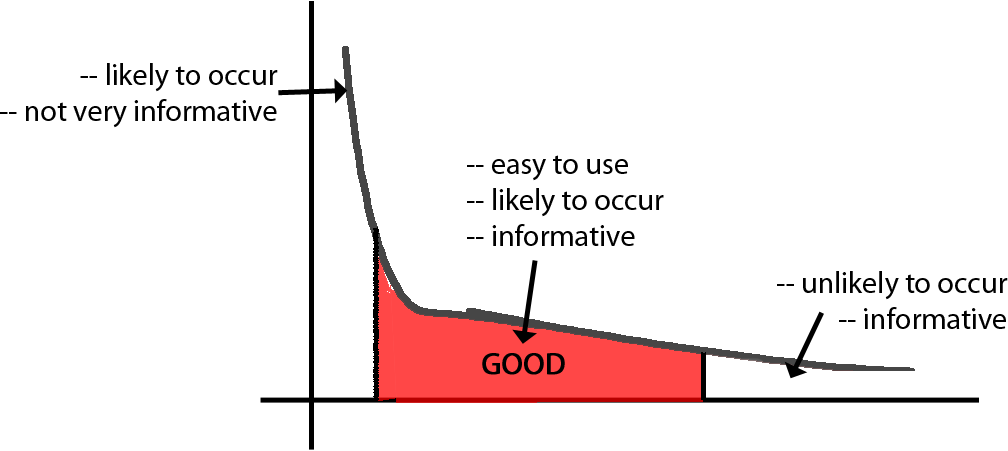
\includegraphics[scale=0.3]{figures/frequency-cutoff.png}
	\caption{Space of features which are both informative and relatively frequent (very useful!). Typical result of applying stoplist and using frequency cut-off.}
	\label{fig:frequency-cutoff}
\end{figure}

\subsubsection{Mutual Information Cutoff}

\textbf{Mutual information} (see Section \ref{sec:mutual-information}) can be used to select good features. To select $k$ good" features, compute the mutual information of each word in the training corpus, order them from highest to lowest with respect to MU and choose the first $k$. Figure \ref{fig:example-mu} shows the words with the highest mutual information for different classes of documents in the \textbf{Reuters corpus}. Notice how there are no stop words, and all the words are clearly relevant to the associated class.

\begin{figure}[H]
	\centering
	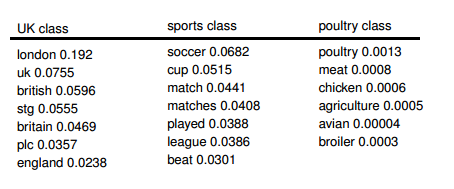
\includegraphics[scale=0.7]{figures/mutual-information-cutoff.png}
	\caption{Three Classes in Reuters Corpus and the Words with Highest Mutual Information}
	\label{fig:example-mu}
\end{figure}

This can \textbf{greatly increase classification accuracy}, much more so than frequency cutoff. This is shown in Figure \ref{fig:mu-acc-impact}, which shows the accuracy of classifiers with different values for $k$. Too high a value for $k$ hurts the classification, as irrelevant features start to be used. Too low a value and not enough features are used to accurately distinguish between the different classes.

\begin{figure}[H]
	\centering
	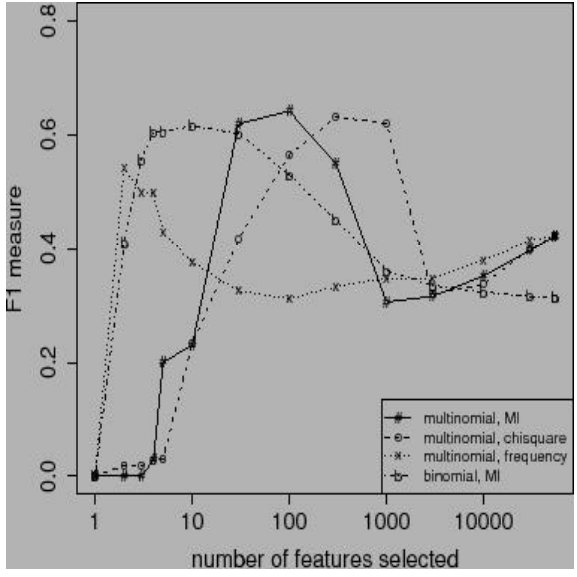
\includegraphics[scale=0.4]{figures/feature-amount-performance.png}
	\caption{Impact of Number of Features on Accuracy}
	\label{fig:mu-acc-impact}
\end{figure}

\subsection{Multi-class Text Classification}

Rather than saying whether a document is about China or not, what if we wanted to know if a document is about China, Japan, South or North Korea? Each of the four countries would be a class, so we have \textbf{multiclass} classification, instead of \textbf{binary} classification.

Even though Naive Bayes is inherently a binary classifier, we can use it for multiclass classification. We build a Naive Bayes classifier $\gamma_c$ for each class $c \in C$. When we want to classify a test document $d$, we run $d$ through each classifier and assign $d$ the class $c$ for all $c$ in which $\gamma_c$ returns true.

If you want to build a classifier which assigns \textbf{only one class} to a document, then simply run the classification as before and choose the class $c$ with the \textbf{highest score (highest probability)} out of all the classes where $\gamma_c$ returns true.

See Section \ref{sec:multiclass-classifier-evaluation} for ways to evaluate multiclass classifiers.

\section{Semantic Similarity}

Suppose you want to group words according to how similar they are. For example, you may group "apple", "orange" and "banana" together, as they're all edible fruit. How is it possible to do this automatically, just by processing text How do you \textbf{measure} the similarity of two words? Two words are similar if their meaning is roughly the same. That is, they're \textbf{semantically} similar.

\subsection{Vector Space Model}

The \textbf{Vector Space Model} can be used to determine the similarity of two words, just like how it was used for IR. It makes the assumption that word meaning $\approx$ context; that is, words mean similar things if they are \textbf{used in similar contexts}. The model represent words as vectors in multidimensional space. Words whose vectors are \textbf{closer in space} are more similar to each other.

Figure \ref{fig:vector-space-model} shows a collection of words represented in vector space. Here, "storage" is more similar to "disk" than "shuttle", because the vector that represents "storage" is \textit{closer} to the vector that represents "disk" than "shuttle"'s disk. This model raises an important question -- \textbf{how are these vectors constructed?}

\begin{figure}
	\centering
	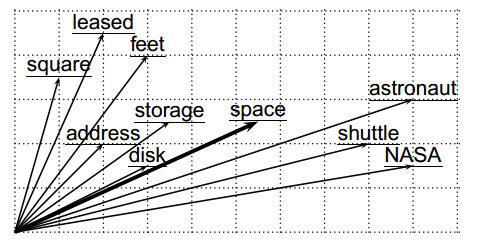
\includegraphics[scale=0.6]{figures/vector-space-model.png}
	\caption{Documents Represented as Vectors in Multidimensional Space}
	\label{fig:vector-space-model}
\end{figure}

Let $W$ be all the words in the vocabulary and $n = |W|$ be the number of words. Each word is represented by an $m$-dimensional vector, where $m$ is the number of context words, or features. \textbf{Context words} are words specifically chosen to be used for extracting semantics.  Each \textbf{component} of the $m$-dimensional vector is an \textbf{association measure} of the word the vector is representing and the context word that component refers to. 

Here, a \textbf{co-occurrence vector} is used to represent a word. This vector contains an association measure between a word and all the context words, based on \textbf{how many times the two words appear together}. This measures how often a word is used in a particular context, so once you have that you can check the contexts two words are used in to be if they're used in similar ones (thus, they are similar).

\paragraph{\textbf{NOTE:} } You could use an $n$-dimensional vector to represent all $n$ words, which each component being an association measure of two words. However, this is very expensive computationally and storage-wise.
\paragraph{}

To construct an association measure between a word and context word, a \textbf{predefined window} of words is often considered for the context. Let $d$ be the size of the window. This means that, for each occurrence of word, look $\frac{d}{2}$ words before it and $\frac{d}{2}$ after. Then, count the \textbf{number of times each context word appears in those windows}, and use that frequency as the association measure.

Suppose we have a vocabulary of three \textbf{words} -- "first", "learning" and "discovering". We have five \textbf{context words} -- "these", "meaning", "the", "practical", "come". Suppose we are using a window size of 6 ($d = 3$) and examining the text below. We look for each occurrence of a word in the vocabulary and count the number of times context words appear in that window. After doing this, we're left with Table \ref{tab:vsm-co-occurrence-vectors}, which represents each of the three words as 5-dimensional \textbf{co-occurrence} vector.

\begin{quote}
"And this is the last thing the anthropologist who tries to understand symbols can afford to do. He must start with the explanations and commentaries which his informants themselves offer about their \textit{"symbols. These must \textbf{first} be examined in"} the contexts in which they are usually employed, where they occur naturally, although subsequent generalizing discussion helps the anthropologist to improve his very \textit{"superficial initial standing. \textbf{Learning} the meaning of"} symbols is part of the \textit{"anthropologist's practical semantics: \textbf{discovering} the meaning of"} words, noticing when their use is appropriate and when it is not. all this requires imagination, patience, considerable linguistic skill, but above all a rigorous respect for the facts. \textit{"These must come \textbf{first}; fantasy can come"} later"
\end{quote}

\paragraph{\textbf{NOTE:}} Context windows are italicised and the occurrences of regular words are emboldened.

\paragraph{}

\begin{table}[H]
	\centering
	\begin{tabular}{|r|l|l|l|l|l|}
		\hline
		& these & meaning & the & practical & same \\
		\hline
		first & 2 & 0 & 0 & 0 & 2 \\
		learning & 0 & 1 & 1 & 0 & 0 \\
		discovering & 0 & 1 & 1 & 1 & 0 \\
		\hline
	\end{tabular}
	\caption{Three words represented as co-occurrence vectors with respect to five context words}
	\label{tab:vsm-co-occurrence-vectors}
\end{table}

The steps of constructing a vector space model to measure word similarity are as follows:
\begin{enumerate}
	\item Determine a \textbf{set of context words} -- an example of this is selecting the $k$ most frequent words in the corpus
	\item Determine a \textbf{window size} -- e.g. 10 words (5 to the left and 5 to the right)
	\item Compute \textbf{co-occurrence vector} for each word in corpus -- this uses an \textbf{association measure} (Section \ref{sec:association-measures}, such as how many often a word co-occurs with context words in the given window
	\item Use a \textbf{similarity measure} (Section \ref{sec:similarity-measures} to compute whether vectors are close in space (i.e. words are similar)
\end{enumerate}

\subsection{Variations}

\textbf{Stop words (function words)} could be eliminated as \textbf{context words}, as they're often used near \textit{most} words at some point and have little semantic meaning. Therefore, they just add noise to the final similarity measure. Additionally, the \textbf{roots/stems} of words could be used instead of the word itself, which adds a layer of generalisation to the association.

The \textbf{size of the context} (window size) has a big impact on how words are associated to one another. Small windows (e.g. 2) result in \textbf{paradigmatic} associations, which means words are seen as similar if they are the same type/category of word (e.g. words are both vehicles, fruit, pets, etc.). Large windows (e.g. 30) result in \textbf{syntagmatic} associations which relate worlds that are part of the same high-level topic. This is shown in Figure \ref{fig:size-of-context-effect}, where "car" is similar to "van", "truck", etc. with a 2-word window but is related to more broader concepts with a 30-word window, such as "drive" and "park".

\begin{figure}
	\centering
	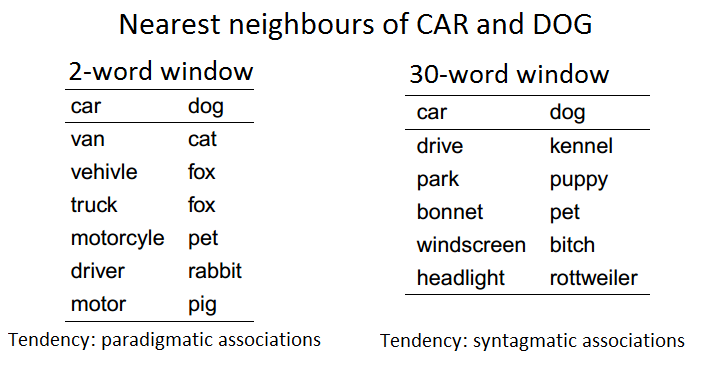
\includegraphics[scale=0.55]{figures/size-of-window.png}
	\caption{Effect of Different Sizes for Context Window}
	\label{fig:size-of-context-effect}
\end{figure}

\subsection{Association Measures}
\label{sec:association-measures}

There many different association measures that could be used to link words to context words:
\begin{itemize}
	\item \textbf{Binary Co-occurrence} -- 0 if word has \textit{never} occurred with the context word and 1 if it has at least once
	\item \textbf{Co-occurrence Frequency} -- as discussed before, this is the number of times the context word has appeared in the word's \textbf{context window}
	\item \textbf{Pointwise Mutual Information (PMI)} -- uses concept of information to associate word with context word (see Section \ref{sec:mutual-information}). See Table \ref{tab:pmu-association-example} for PMI. Notice how words like "Pepsi" are associated much more to "drink" than "it", even though it co-occurs less. This is because the PMI measure has considered the fact that "it" is more common and co-occurs with many other words as well (whereas "Pepsi" will co-occur with less).
\end{itemize}

\begin{table}
	\centering
	\begin{tabular}{|l|l|l|}
		\hline
		\textbf{Object} & \textbf{Co-occurrence Count} & \textbf{PMI} \\
		\hline
		tea & 4 & 11.75 \\
		Pepsi & 2 & 11.75 \\
		beer & 5 & 10.20 \\
		much & 3 & 2.54 \\
		it & 3 & 1.24 \\
		\hline
	\end{tabular}
	\caption{Words co-occurring with context word "drink" and their PMI association measure (Hindle, 1990)}
	\label{tab:pmu-association-example}
\end{table}

\subsection{Similarity Measures}
\label{sec:similarity-measures}

Each word is represented as a vector of $m$ values -- $\vec{x} = (x_1, x_2, ..., x_m)$. $\vec{x}$'s components contain association measures of the word represent by $\vec{x}$ to all $m$ context words. Therefore, to determine the similarity between two words we perform some operation on the two words' vectors. This is the \textbf{similarity measure} $s(\vec{x}, \vec{y})$.

The \textbf{Euclidean distance} between two vectors $\vec{x}$ and $\vec{y}$ is given in Equation \ref{eq:euclidean-distance-sim}. The \textbf{cosine} of the angle between two vectors $\vec{x}$ and $\vec{y}$ is given in Equation \ref{eq:cosine-similarity-duplicate}. The former measures how close/far apart two vectors are and the latter measures the angle between two two vectors. Both of the these are commonly used as the similarity measure. \textbf{Cosine similarity} tends to be used more however.

\begin{equation}
	|\vec{x} - \vec{y}| = \sqrt{ \sum_{i=1}^n {x_i - y_i}^2 }
	\label{eq:euclidean-distance-sim}
\end{equation}
\begin{equation}
	cos(\vec{x}, \vec{y}) = \frac{\vec{x} \cdot \vec{y}}{|\vec{x}| |\vec{y}|}
	\label{eq:cosine-similarity-duplicate}
\end{equation}

Suppose we have five words in the vocabulary -- "cosmonaut", "astronaut", "moon", "car", "truck" -- and the context words are these same five words. Using co-occurrence frequency as the association measure, considering all context windows gives us the vectors in Table \ref{tab:similarity-measure-example}.

Using the cosine of the angle between vectors as the similarity measure, the similarity of "cosmonaut" and "moon", as well as "cosmonaut" and "truck", are given in Equation \ref{eq:similarity-measure-example}.

\begin{table}
	\centering
	\begin{tabular}{|r|l|l|l|l|l|}
		& \textbf{cosmonaut} & \textbf{astronaut} & \textbf{moon} & \textbf{car} & \textbf{truck} \\
		\textbf{cosmonaut} & 2 & 0 & 1 & 1 & 0 \\
		\textbf{astronaut} & 0 & 1 & 1 & 0 & 0 \\
		\textbf{moon} & 1 & 1 & 2 & 1 & 0 \\
		\textbf{car} & 1 & 0 & 1 & 3 & 1 \\
		\textbf{truck} & 0 & 0 & 0 & 1 & 2 \\								
	\end{tabular}
	\caption{Co-occurrence frequency of five words with each other}
	\label{tab:similarity-measure-example}
\end{table}

\begin{equation}
\begin{aligned}[b]
	cos(\vec{cosmonaut}, \vec{moon}) = 
	\frac{\vec{cosmonaut} \cdot \vec{moon}}{|\vec{cosmonaut}| |\vec{moon}|}
	&= \frac{2 \cdot 1 + 0 \cdot 1 + 1 \cdot 2 + 1 \cdot 1 + 0 \cdot 0}{ \sqrt{2^2 + 0^2 + 1^2 + 1^2 + 0^2} \sqrt{1^2 + 1^2 + 2^2 + 1^2 + 0^2} } \\
	&= \frac{5}{\sqrt{6}\sqrt{7}} = \frac{5}{6.481} = 0.77 \\
	\\
	cos(\vec{cosmonaut}, \vec{truck}) = 
	\frac{\vec{cosmonaut} \cdot \vec{truck}}{|\vec{cosmonaut}| |\vec{truck}|}
	&= \frac{2 \cdot 0 + 0 \cdot 0 + 1 \cdot 0 + 1 \cdot 1 + 0 \cdot 2}{ \sqrt{2^2 + 0^2 + 1^2 + 1^2 + 0^2} \sqrt{0^2 + 0^2 + 0^2 + 1^2 + 2^2} } \\
	&= \frac{1}{\sqrt{6}\sqrt{5}} = \frac{1}{5.477} = 0.18 \\
	\label{eq:similarity-measure-example}
\end{aligned}
\end{equation}

Therefore, because the similarity measure for "cosmonaut" and "truck" is \textbf{smaller} than "cosmonaut" and "moon", "cosmonaut" and "moon" are more similar to each other than "cosmonaut" and "truck". 

\section{Evaluation Measures}

\subsection{Information Retrieval}
\label{sec:ir-evaluation}

\textbf{Evaluation} of information retrieval systems is typically done using two main measurements -- precision and recall. \textbf{Recall} is the proportion of \textit{relevant} documents returned out of all the relevant documents that exist. \textbf{Precision} refers to the proportion of returned documents that are actually relevant (how \textit{precise} is the result). These values range from 0 to 1, where 1 is maximum recall/precision and 0 is none. Figure \ref{fig:recall-precision-vis} illustrates what recall and precision mean.

\begin{figure}
	\centering
	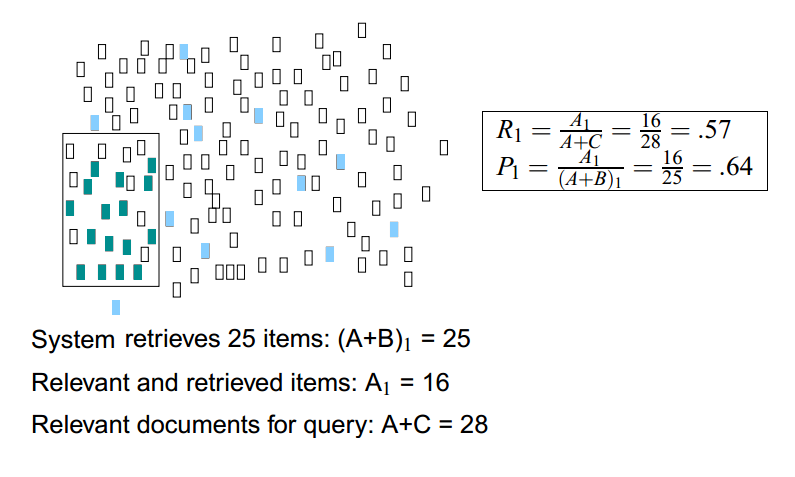
\includegraphics[scale=0.45]{figures/precision-recall.png}
	\caption{Illustration of Precision and Recall for a Particular System}
	\label{fig:recall-precision-vis}
\end{figure}

To compute these values, a \textbf{contingency table} must first be computed. This records the number of times the IR system:
\begin{itemize}
	\item retrieved a document that was \textit{was} relevant
	\item retrieved a document when it \textit{wasn't} relevant
	\item \textit{did not} retrieved a document that was \textit{was} relevant
	\item \textit{did not} retrieved a document when it \textit{wasn't} relevant
\end{itemize}
An example of this is given in Table \ref{tab:example-contingency}.

\begin{table}[H]
	\centering
	\begin{tabular}{|r|l|l|l|}
		\hline
		& \textbf{Relevant} & \textbf{Non-relevant} & \textbf{Total} \\
		\hline
		\textbf{Retrieved} & $N_{11}$ & $N_{10}$ & $N_{11} + N_{10}$ \\
		\textbf{Not Retrieved} & $N_{01}$ & $N_{00}$ & $N_{01} + N_{00}$ \\
		\hline
		\textbf{Total} & $N_{11} + N_{01}$ & $N_{10} + N_{00}$  & $N_{11} + N_{01} + N_{10} + N_{00}$ \\
		\hline
	\end{tabular}
	\caption{Frequency/Contingency Table for Class One}
	\label{tab:example-contingency}
\end{table}

Equations \ref{eq:recall} and \ref{eq:precision} show how to compute recall and precision respectively, using the contents of the contingency table.

\begin{equation}
	\frac{N_{11}}{N_{11} + N_{01}}
	\label{eq:recall}
\end{equation}

\begin{equation}
	\frac{N_{11}}{N_{11} + N_{10}}
	\label{eq:precision}
\end{equation}

\textbf{F-measure} combines both precision and recall into a single measurement. The formula is given in Equation \ref{eq:f-measure}, where $R$ is recall, $P$ is precision and $\alpha \in [0..1]$ determines how heavily the measurement weights precision and recall. \textbf{High} $\alpha$ makes \textbf{recal}  more important and \textbf{low} $\alpha$ makes \textbf{precision} more important. The most common value for $\alpha$ is 0.5 ($F_{0.5} = \frac{2PR}{P + R}$).

\begin{equation}
	F_{\alpha} = \frac{1}{\alpha \frac{1}{P} + (1-\alpha)\frac{1}{R}}
	\label{eq:f-measure}
\end{equation}

\subsubsection{Precision Cutoff}

Recall and precision change depending on the number of relevant documents returned by the IR system.

Take the example in Figure \ref{fig:precision-cutoff}. The precision for the first ranking after running through the \textbf{first five documents in order} is 1.0. The second ranking has a precision of 0, since the first five documents are all non-relevant (but there are five relevant documents after that!) When counting relevant/non-relevant documents through the \textit{entire} ordered document list, the precision will be same regardless of order.

\textbf{Precision cut-off} is when you only return a pre-defined \textbf{maximum} of documents. This may improve precision, but recall is reduced (as less documents are returned). Therefore, it is important to \textbf{tweak} the point at which you stop counting to optimise recall and precision to where you want them. Too short a cut-off and precision may appear \textit{low}, as it hasn't had a chance to sample enough returned documents. Too long and there will be many irrelevant documents, which will also result in low precision.

\begin{figure}[H]
	\centering
	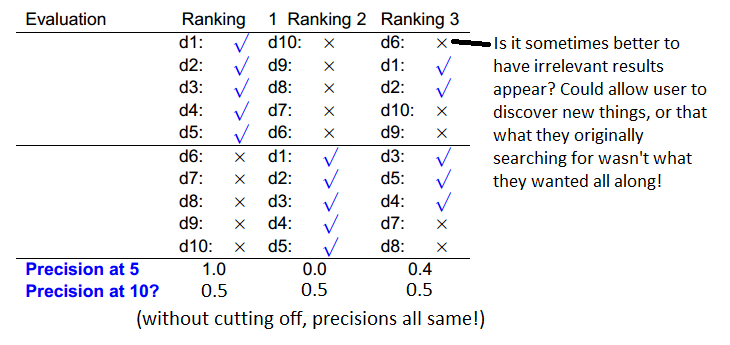
\includegraphics[scale=0.4]{figures/precision-cutoff.png}
	\caption{Illustration of how decision on where to cut-off results has an effect on the evaluation of the IR system}
	\label{fig:precision-cutoff}
\end{figure}

\textbf{Average precision} is another way of measuring precision, which \textbf{averages} the precision measurements from using different cut-off values.An example of this is shown in Figure \ref{fig:average-precision}.

\begin{figure}[H]
	\centering
	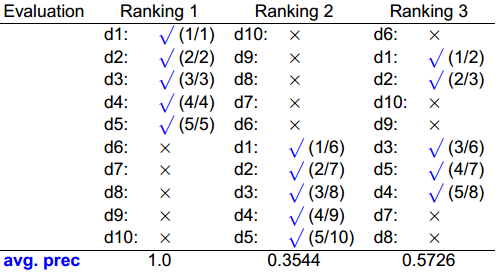
\includegraphics[scale=0.4]{figures/average-precision.png}
	\caption{Computing average precision by taking slices of results}
	\label{fig:average-precision}
\end{figure}

\subsection{Binary Classification}

When you have two classes, evaluating classifiers is done in the same way as information retrieval systems. You create a $2 \times 2$ \textbf{contingency table} and then use the values inside it to compute the precision, recall and F-measure. This is shown in Table \ref{tab:bin-classify-example-contingency} and Equations \ref{eq:bin-classify-recall} and \ref{eq:bin-classify-precision}. $t_p$ and $t_n$ are the number of \textbf{true} positives and negatives, while $f_p$ and $f_n$ are the number \textbf{false} positives and negatives.

\begin{table}[H]
	\centering
	\begin{tabular}{|r|l|l|}
		\hline
		& \textbf{Real Class = Yes} & \textbf{Real Class = No} \\
		\hline
		\textbf{Output Class = Yes} & $t_p$ & $f_p$ \\
		\textbf{Output Class = No} & $f_n$ & $t_n$ \\
		\hline
	\end{tabular}
	\caption{Contingency Table for Binary Classification}
	\label{tab:bin-classify-example-contingency}
\end{table}

\begin{equation}
	\frac{t_p}{t_p + f_n}
	\label{eq:bin-classify-recall}
\end{equation}

\begin{equation}
	\frac{t_p}{t_p + f_p}
	\label{eq:bin-classify-precision}
\end{equation}

\subsection{Multi-class Classification}
\label{sec:multiclass-classifier-evaluation}

Evaluating the performance of binary classifiers using precision and recall is simple. When you have a classifier which can assign more than two potential classes to a data item, things get a little more complicated.

You can compute the precision and recall \textbf{per class} (say, for each classifier $\gamma_c$), but then how do you \textbf{combine} the multiple performance measures into one?

\textbf{Macroaveraging} computes the performance for each class, then averages the results. \textbf{Microaveraging} collects the \textit{decisions} for all classes, computes a contigency table and \textit{then} evaluates.

To compute \textbf{macroaverage} precision:
\begin{enumerate}
	\item Construct $2 \times 2$ frequency table for each class $c \in C$
	\item Compute precision of each class table
	\item Compute average precision from individual precisions
\end{enumerate}

To compute \textbf{microaverage} precision:
\begin{enumerate}
	\item Construct $2 \times 2$ frequency table for each class $c \in C$
	\item Sum entries of all tables together to create a new table
	\item Compute precision using values in combined table
\end{enumerate}

Example of computing microaverage and macroaverage for a two-class problem is given below. Tables \ref{tab:multiclass-eval-class1} \ref{tab:multiclass-eval-class2} show the frequency tables (and precision of them) for the two classes and \ref{tab:multiclass-eval-classsum} is the sum of the two tables (for computing microaverage).

\begin{table}[H]
	\centering
	\begin{tabular}{|r|l|l|}
		\hline
		& is class & is not class \\
		\hline
		classifier output = "yes" & $N_{11} = 10$ & $N_{10} = 10$ \\
		classifier output = "no" & $N_{01} = 10$ & $N_{00} = 970$ \\
		\hline
		\textbf{Precision} & \multicolumn{2}{l|}{
			$\frac{N_{11}}{N_{10}} = \frac{10}{10 + 10} = \frac{10}{20} = 0.5$
		} \\
		\hline
	\end{tabular}
	\caption{Frequency/Contingency Table for Class One}
	\label{tab:multiclass-eval-class1}
\end{table}

\begin{table}[H]
	\centering
	\begin{tabular}{|r|l|l|}
		\hline
		& is class & is not class \\
		\hline
		classifier output = "yes" & $N_{11} = 90$ & $N_{10} = 10$ \\
		classifier output = "no" & $N_{01} = 10$ & $N_{00} = 890$ \\
		\hline
		\textbf{Precision} & \multicolumn{2}{l|}{
			$\frac{N_{11}}{N_{10}} = \frac{90}{90 + 10} = \frac{90}{100} = 0.9$
		} \\
		\hline
	\end{tabular}
	\caption{Frequency/Contingency Table for Class Two}
	\label{tab:multiclass-eval-class2}
\end{table}

\begin{table}[H]
	\centering
	\begin{tabular}{|r|l|l|}
		\hline
		& is class & is not class \\
		\hline
		classifier output = "yes" & $N_{11} = 100$ & $N_{10} = 20$ \\
		classifier output = "no" & $N_{01} = 20$ & $N_{00} = 1860$ \\
		\hline
		\textbf{Precision} & \multicolumn{2}{l|}{
			$\frac{N_{11}}{N_{10}} = \frac{100}{100 + 20} = \frac{100}{120} = 0.83$
		} \\
		\hline
	\end{tabular}
	\caption{Micro-averaged Frequency/Contingency Table (Sum of Tables \ref {tab:multiclass-eval-class1} and \ref{tab:multiclass-eval-class2})}
	\label{tab:multiclass-eval-classsum}
\end{table}

The macroaverage is the average precision of all individual contingency tables, which takes it $\frac{0.5 + 0.9}{2} = 0.7$. The microaverage is the precision of the contingency table constructed by summing the individual contingency tables, which is $\frac{100}{100 + 20} = \frac{100}{120} = 0.83$.

Notice how these are measures are \textbf{significantly different}. The microaveraged precision is \textbf{dominated} by the score on the \textbf{common classes}. This means if you perform really well on rare classes and poorly on common classes, the precision is lower. The macroaverage precision weights the performance on all classes \textbf{equally}, so if rare classes are classified correctly, then the precision is increased.

If you only choose one measure to evaluate the performance of your multi-class classifier, then be sure to think it through carefully. If classifying common classes accurately is more important to use, then use microaveraging. If you don't care about that and you care about all classes equally (e.g. you just didn't have that much of one class in a test dataset, but you still care about it as much), then use macroaveraging. Alternatively, you can always just compute both and use the results from both to determine the effectiveness of the classifier.

\section{$n$-Gram Modelling}
\label{sec:ngram-modelling}

Up to now, all the techniques that have been covered involved counting individual words, which also used the Bags of Words model. The probabilities of word \textit{sequences} (i.e. sentences) can be computed, which creates a \textbf{probabilistic language model}. This model can be applied to various tasks, such as:
\begin{itemize}
	\item speech recognition
	\item handwriting recognition
	\item context-sensitive spelling correction
	\item word completion for texting
\end{itemize}

To predict what word is next, we can use a \textbf{history-based model}, in which we predict following things from past things (history $\approx$ context).  But how far in history do we go back? The \textbf{Markov assumption} states that $w_i$ only depends on \textit{immediately} preceding tokens. How many tokens you look back at is the \textbf{order} of the Markov assumption:
\paragraph{}
\begin{tabular}{rll}
\textbf{0th order} &(Unigram) & $P(w_i|w_1...w_{i - 1}) \approx P(w_i)$ \\
\textbf{First order} & (Bigram) & $P(w_i|w_1...w_{i - 1}) \approx P(w_i|w_{i-1}) = \frac{P(w_{i-1}w_i)}{P(w_{i-1})}$ \\
\textbf{Second order} & (Trigram) & $P(w_i|w_1...w_{i - 1}) \approx P(w_i|w_{i-2}w_{i-1})$ \\
\end{tabular}

An $n$-gram is a continuous sequence of $n$ words. Building a language model using $n$-grams requires the $(n - 1)$th order Markov assumption. These language models are also known as \textbf{Markov models}.

Equation \ref{eq:ngram-for-sentences} shows how you can \textbf{compute the probability of a sentence} using a \textbf{bigram language model}. Note that the first word just uses its own probability as there is no previous word. Figure \ref{fig:bigram-model} shows a graphical representation of the model. Each word is a node, which the word itself in the centre of it. Moving from $w_1$ to $w_2$ adds a multiplier to the final sequence probability; each time you move to the next node $w_j$ from $w_i$ a new multiplier is applied. These multipliers are determined by the probability of the bigram composed by the words $w_i$ and $w_j$, until we reach the end the sentence.

\begin{figure}
	\centering
	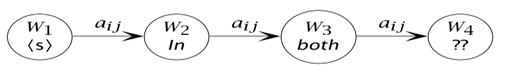
\includegraphics[scale=0.5]{figures/bigram-chain.png}
	\caption{Markov model for word sequence probabilities using bigrams}
	\label{fig:bigram-model}
\end{figure}

\begin{multline}\\
	P(\text{He often wears tight trousers}) \approx \\
	P(\text{He}) \cdot P(\text{often$|$He}) \cdot P(\text{wears$|$often}) \cdot P(\text{tight$|$wears}) \cdot P(\text{trousers$|$tight})
	\label{eq:ngram-for-sentences}
\\\end{multline}

Bigram models have been tremendously successful, even though they only look one token back. This is because \textbf{long-distance dependencies} between words, like the one in Figure \ref{fig:long-distance-dependency} are rare. 74\% of all dependencies in the Penn Treebank are with an \textbf{adjacent} word, which can be captured by bigrams. This is not always the case however. The 26\% of other dependencies are still lost with bigrams, as evident by the example Figure \ref{fig:long-distance-dependency}. Depending on the text being processed, higher order models (e.g. trigrams) may be required.

\begin{figure}
	\centering
	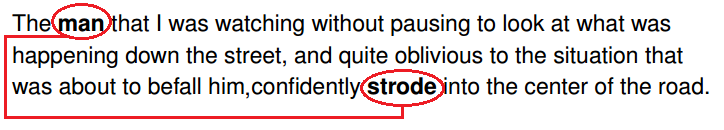
\includegraphics[scale=0.5]{figures/long-distance-dependency.png}
	\caption{Long Distance Dependency Between Two Words}
	\label{fig:long-distance-dependency}
\end{figure}

\subsection{Deriving Language Model}

To \textbf{construct} a probabilistic language model in practice, get a corpus and do the following steps:
\begin{enumerate}
	\item Start with a \textbf{vocabulary} $V$ (token types), which can be:
	\begin{itemize}
		\item all word types in corpus
		\item $k$th most frequent word types in corpus
		\item word types with highest mutual information with document classes (topic classification)
	\end{itemize}
	\item Pick a \textbf{model type}, such as unigrams, bigrams, trigrams, etc.
	\item Estimate the \textbf{parameters}, or \textbf{word/sequence probabilities}. This is typically done using \textbf{frequency counts}
\end{enumerate}

The probabilities of each word/sequence is the \textbf{relative frequency}. Equations \ref{eq:unigram-prob}, \ref{eq:bigram-prob} and \ref{eq:trigram-prob} show hot to compute the probabilities of unigrams, bigrams and trigrams of occurring respectively. $N$ is the number of words in the entire corpus, $f(w_i)$ is the frequency of word $w_i$ in the corpus and $f(w_1, w_2, ..., w_n)$ is the frequency of sequence $w_1w_2...w_n$ occurring in the corpus.

\begin{equation}
	P(w_1) = \frac{f(w_1)}{N}
	\label{eq:unigram-prob}
\end{equation}
\begin{equation}
	P(w_2|w_1) = \frac{f(w_1, w_2)}{f(w_1)}
	\label{eq:bigram-prob}
\end{equation}
\begin{equation}
	P(w_3|w_1,w_2) = \frac{f(w_1, w_2, w_3)}{f(w_1, w_2)}
	\label{eq:trigram-prob}
\end{equation}

Figure \ref{fig:brown-bigram-model} shows part of a bigram model generated from the \textbf{Brown} corpus, which has one million words. Figure \ref{fig:bnc-bigram-model} shows part of a bigram generated from the \textbf{BNC} corpus, with 100 million tokens. Notice how these models are being represented by \textbf{frequency tables}, where the entry at row $i$ and column $j$ is the number of times the bigram $w_i w_j$ occurred in the corpus.

\begin{figure}
	\centering
	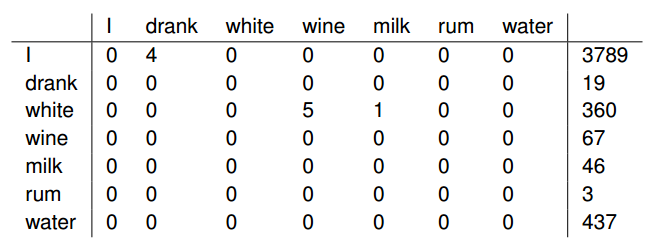
\includegraphics[scale=0.5]{figures/brown-bigram-model.png}
	\caption{Bigram Probability Model Derived from Brown Corpus (rows are first word in bigram)}
	\label{fig:brown-bigram-model}
\end{figure}

\begin{figure}
	\centering
	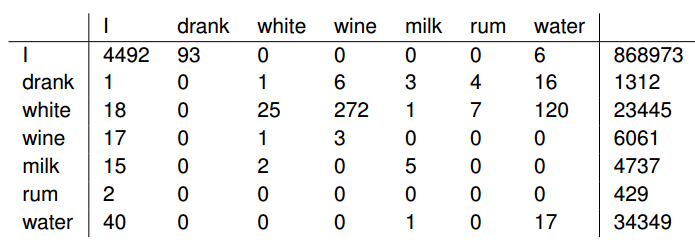
\includegraphics[scale=0.5]{figures/bnc-bigram-model.png}
	\caption{BNC Probability Model Derived from BNC (rows are first word in bigram)}
	\label{fig:bnc-bigram-model}
\end{figure}

\subsection{Smoothing}

In the ideal scenario, higher $n$ (meaning higher order $n$-grams) means more discrimination (more accurate results). The same works for corpora -- bigger corpora work better than small ones. However, the higher $n$ is, the more \textbf{data sparseness} we have. Data sparseness means more zero probabilities, which lead to \textbf{complete failure} when predicting the next work in a sequence , or computing the probability of a sentence.

The problem with using such a language model is that it is surprised when unseen $n$-grams appear ($P(unseen) = 0$). This happens often, especially if $n$ is high. Data sparseness means that, not only is the probability of zero count words too \textit{low}, but the probability of nonzero count words is too \textbf{high]}.

This problem can be solved by \textbf{smoothing}, which re-evaluates the zero-probability and low-probability $n$-grams and assign them \textbf{non-zero values}. This addresses data sparseness and prevents the model from completely breaking down.

\textbf{Laplace's law} is one method of smoothing, which simply adds one to each frequency. To keep the balance, the vocabulary size is added to the denominator used to compute the probability. Laplace smoothing applied to the probability of aw \textbf{word sequence of length $n$} is given in Equation \ref{eq:laplace-n-sequence}. Laplace applied to the probability of a \textbf{bigram} is given in Equation \ref{eq:laplace-bigram}. $N$ is the length of the corpus and $V$ is the vocabulary size.

\begin{equation}
	P_{+1}(w_1,w_2,...,w_n) = \frac{f(w_1,w_2,...,w_n) + 1}{N + V^{n}}
	\label{eq:laplace-n-sequence}
\end{equation}

\begin{equation}
	P_{+1}(w_2|w_1) = \frac{f(w_1,w_2) + 1}{f(w_1) + V}
	\label{eq:laplace-bigram}
\end{equation}

What happens if $N$ or $V$ is very large? Then you start \textbf{assigning too high probabilities to unseens}. A quick fix to this is \textbf{Lidstone's law}, which reduces the denominators magnitude by $\lambda$, as shown in Equations \ref{eq:lidstone-n-sequence} and \ref{eq:lidstone-bigram}.

\begin{equation}
	P_{+\lambda}(w_1,w_2,...,w_n) = \frac{f(w_1,w_2,...,w_n) + \lambda}{N + \lambda V^{n}}
	\label{eq:lidstone-n-sequence}
\end{equation}

\begin{equation}
	P_{+\lambda}(w_2|w_1) = \frac{f(w_1,w_2) + \lambda}{f(w_1) + \lambda V}
	\label{eq:lidstone-bigram}
\end{equation}

This prevents us from assigning too much probability mass to unseens, providing we find a good estimate for $\lambda$ (which requires trial and error).

How do you compute the likelihood of encountering a \textbf{new, unseen word type} in the future? You could simply assign a probability of 0, or add one, but we can do more. Let $N_r$ be the number of $n$-grams with frequency $r$, so $N_0$ is the number of $n$-grams with frequency 0, $N_1$ is the number of $n$-grams with frequency 1 and so on. This makes $N = \sum_{r} {N_r}$ the total number of $n$-grams.

\textbf{Good-Turing smoothing} uses the \textbf{proportion of singletons} ($n-$-grams $\in N_1$) to estimate the \textbf{proportion of unseen words} ($n-$-grams $\in N_0$). It does this by \textbf{not using standard relative frequency}. Instead, it uses Equation \ref{eq:good-turing-smoothing} to estimate the probability of an $n$-gram in $N_r$, for all $r$. Notice how unseen $n$-grams are \textbf{special cases} that use a different formula (proportion of $n$-grams seen once to all $n$-grams).

\begin{equation}
	r^{\ast} = \begin{cases}
		\frac{N_1}{N},& \text{if }r=0 \\
		(r + 1)\frac{N_{r+1}}{N_r} ,& \text{if }r>0
	\end{cases} \;\;\;\; \forall \; r
	\label{eq:good-turing-smoothing}
\end{equation}

Smoothing methods typically try to "squeeze" more information out of the given data. But what about  \textbf{adding more data}? \textbf{Web-based smoothing} uses vast amounts of data automatically collected from the web. The web counts are used to compute $n$-gram probabilities if the original counts resulted in an \textbf{unreliable prediction} (model broke down because of zero probabilities).

\section{Information Theory}

The best evaluation of a language model is using it for a task and then deriving accuracy/precision/recall. An alternative way is to think of evaluation as:
\begin{quote}
	How well does a language model \textbf{predict} some unseen text $T$?
\end{quote}
Additionally, how much \textbf{new} information is in $T$? How surprised is the model to see $T$?

To measure these aspects, we need \textbf{information theory}. This is used for data compression and transmission, and involves the concept of entropy.

\subsection{Information and Entropy}

$X$ is a source of "messages", with a probability distribution $p(x)$. How much new \textbf{information} does a message $x$ contain? Let $I(x)$ be the amount of information a message $x$ contains. The \textbf{less probable} a message is, the \textbf{more information} it contains.

If $x$ and $y$ are two \textbf{independent messages}, then the information gained from knowing both of them is $I(x, y) = I(x) + I(y)$.

$p(x)$  being similar to $p(y)$ \textbf{implies} $I(x)$ is similar to $I(y)$. That is, if two the probability of two messages is similar, then the information gained from individually knowing each will be similar.

\textbf{Entropy} measures the \textbf{average/expected} amount of information in \textit{any} random variable from a message source $X$. For\textit{discrete} probability distributions, it can be computed either formula in Equation \ref{eq:entropy}.
\begin{equation}
	\begin{aligned}[b]
		H(X) = -\sum_{x \in X} { p(x) \log_2 p(x) } \\
		H(X) = \sum_{x \in X} { p(x) \log_2 {\frac{1}{p(x)}} } \\
		\text{where }0\log0 = 0
	\end{aligned}
	\label{eq:entropy}
\end{equation}

If you already know the \textbf{information gained} from each variable, then Equation \ref{eq:entropy-with-information} can be used.

\begin{equation}
	H(X) = \sum_{x \in X} { p(x)I(x) }
	\label{eq:entropy-with-information}
\end{equation}

An output of 1 means we are completely \textbf{uncertain}, whereas an entropy of 0 means we are completely \textbf{certain} about the value (it is known -- no randomness). Entropy is measured in \textbf{bits}, so it represents the average length of a message to transmit the outcome (value) of a variable.

\paragraph{\textbf{EXAMPLE: Coin}} What is the entropy of flipping each of the following three coins, given the likelihood of it landing heads or tails ($X = \lbrace Head, Tail \rbrace$)?
\paragraph{}
\begin{tabular}{ll}
	Coin 1: & $p(Head) = p(Tail) = 0.5$ \\
	Coin 2: & $p(Head) = 0 \; ; \; p(Tail) = 1$ \\
	Coin 3: & $p(Head) = \frac{3}{4} \;\; ; \;\; p(Tail) = \frac{1}{4}$ \\
\end{tabular}
\paragraph{}

Coin 1 (completely uncertain):
\begin{equation}
\begin{aligned}[b]
	H(X) = \sum_{x \in \lbrace Head, Tail \rbrace} { p(x) \log_2 p(x) }
	&= p(Head) \log_2 p(Head) + p(Tail) \log_2 p(Tail) \\
	&= 0.5 \log_2 p(0.5) + 0.5 \log_2 p(0.5) \\
	&= 0.5 \cdot -1 + 0.5 \cdot -1 = -(-0.5 + -0.5) = -(-1) = 1 \;  \text{bit}
\end{aligned}
\end{equation}
Coin 2 (completely certain):
\begin{equation}
\begin{aligned}[b]
	H(X) = \sum_{x \in \lbrace Head, Tail \rbrace} { p(x) \log_2 p(x) }
	&= p(Head) \log_2 p(Head) + p(Tail) \log_2 p(Tail) \\
	&= 0 \log_2 p(0) + 1 \log_2 p(1) \\
	&= 0 \cdot 0 + 1 \cdot 0 = 0 + 0 = 0 \; \text{bits}
\end{aligned}
\end{equation}
Coin 3: (slightly uncertain):
\begin{equation}
\begin{aligned}[b]
	H(X) = -\sum_{x \in \lbrace Head, Tail \rbrace} { p(x) \log_2 p(x) }
	&= p(Head) \log_2 p(Head) + p(Tail) \log_2 p(Tail) \\
	&= 0.75 \log_2 p(0.75) + 0.25 \log_2 p(0.25) \\
	&= 0.75 \cdot -0.415 + 0.25 \cdot -2 = -(-0.311 + -0.5) = -(-0.811) = 0.811 \; \text{bits}
\end{aligned}
\end{equation}

\paragraph{\textbf{EXAMPLE: 8-Sided Die}} Suppose you are reporting t	he result of rolling a fair 8-sided die. Since there is an equal chance of each side coming up, the probabilities are $p(i) = \frac{1}{8}$ where $i = 1,...,8$. Therefore, the entropy is:
\begin{equation}
\begin{aligned}[b]
H(X) &= -\sum_{i=1}^8 p(i) \log_2 p(i) \\
	&= -\sum_{i=1}^8 \frac{1}{8} \log_2 \frac{1}{8} \\
	&= -\log_2 \frac{1}{8} \\
	&= \log_2 8
	\;\;\;\;\;\;\; \text{by law of logorithms} \\
	&= 3\text{ bits}
	\;\;\;\;\;\; \text{because $2^3 = 8$} \\
\end{aligned}
\end{equation}
And it requires 3 bits to encode the result of rolling a die!

\subsection{Joint and Conditional Entropy} 

\textbf{Joint entropy} is the amount of information needed, on average, to specify the value of \textbf{two} discrete random variables. It requires joint probabilities to compute, and is calculated using Equation \ref{eq:joint-entropy}.

\begin{equation}
	H(X, Y) = - \sum_{x \in X} { \sum_{y \in Y} {
		p(x, y) \log_2 p(x, y)
	} }
	\label{eq:joint-entropy}
\end{equation}

\textbf{Conditional entropy} is how much extra information \textbf{you still need} to supply, on average, to communicate $Y$, given that the other party knows $X$. It requires conditional probabilities to compute, and is calculated using \ref{eq:conditional-entropy}.

\begin{equation}
	H(Y|X) = - \sum_{x \in X} { \sum_{y \in Y} {
		p(x, y) \log_2 p(y|x)
	} }
	\label{eq:conditional-entropy}
\end{equation}

Simplified Polynesian is a language that consists of 3 consonants and 3 vowels. In this language, a consonant \textit{must} be paired with a vowel. Based on a large corpus, the \textbf{joint probability table} which describes the likelihood of consonants being paired with vowels (Table \ref{tab:joint-entropy-example}).

\begin{table}
	\centering
	\begin{tabular}{c|c|c|c|c}
		& p & t & k \\
		\hline
		a & $\frac{1}{16}$ & $\frac{3}{8}$ & $\frac{1}{16}$ & $\frac{1}{2}$ \\
		i & $\frac{1}{16}$ & $\frac{3}{16}$ & 0 & $\frac{1}{4}$ \\
		u & 0 & $\frac{3}{16}$ & $\frac{1}{36}$ & $\frac{1}{4}$ \\
		\hline		
		& $\frac{1}{8}$ & $\frac{3}{4}$ & $\frac{1}{8}$ & \\
	\end{tabular}
	\caption{Joint Probabilities of Vowels and Consonants in Simplified Polynesian}
	\label{tab:joint-entropy-example}
\end{table}

Let $V = \lbrace a, i, u \rbrace$ be the vowels and $C = \lbrace p, t, k \rbrace$ be the consonants. Then the \textbf{conditional entropy} of a vowel, \textbf{given} that you know the consonant it's paired with is:
\begin{equation}
	H(V|C) = - \sum_{v \in V} { \sum_{c \in C} {
		p(c, v) \log_2 p(v|c) } } = \frac{11}{8} = 1.475 bits
\end{equation}

\subsection{Chain Rule}

The \textbf{chain rule for probability} is given in Equation \ref{eq:chain-rule-probability}. \textbf{Entropy has also a chain rule}, which is given in \ref{eq:chain-rule-entropy}.

\begin{equation}
	P(A_1,A_2,...,A_n = P(A_1)P(A_2|A_1)P(A_3|A_1,A_2)...P(A_n|A_1,A_2,...,A_{n-1})
	\label{eq:chain-rule-probability}
\end{equation}

\begin{equation}
\begin{aligned}[l]
	H(X,Y) = H(X) + H(Y|X) \\
	X(X_1,X2,...,X_n) = H(X_1) + H(X_2|X_1) +  H(X_3|X_1,X_2) + ... + H(X_n|X_1,X_2,...,X_{n-1})
	\end{aligned}
	\label{eq:chain-rule-entropy}
\end{equation}

\subsection{Cross Entropy}

We don't know the \textit{actual} probability distribution $t$ that generated $t$. We have a model $m$ (approximation) of $t$. We can measure how well our approximated probability distribution departs from \textbf{actual language use} by seeing how \textbf{surprised} our model is to see $T$. The \textbf{better} the model, the \textbf{lower} the cross-entropy. This is called \textbf{cross entropy}, and can be computed using Equation \ref{eq:cross-entropy}. $T$ is the text (with $n$ words) and $m$ is our model approximation.

\begin{equation}
	H(t,m) = \lim_{n \rightarrow \infty} \frac{1}{n} \sum_{W \in T} t(w_1,...,w_n) \log m(w_1, ..., w_n)
	\label{eq:cross-entropy}	
\end{equation}

Entropy can be used to determine how \textbf{uncertain} you are about the next character/word in a text. The entropy rate of a language can be computed using Equation \ref{eq:entropy-language}. $H(X_i)$ are the characters of the language, or every word you have uttered in your life ($26 \times 26$ joint probability table). From human experiments, Shannon estimated the entropy rate of English $H(English)$ to be between 1.25 and 1.35.

\begin{equation}
	H_{rate}(L) = \lim_{n \rightarrow \infty} \frac{1}{n}H(X_1,X_2,...,X_n)
	\label{eq:entropy-language}
\end{equation}

These experiments given an \textbf{upper bound} on true entropy. Table \ref{tab:entropy-rates-of-english} shows the cross entropy of various model. Creating a language model which results in 1.34 entropy is the final goal.

Note that when computing the cross-entropy of a model, be sure to compute it on a \textbf{separate, independent test set}. This is because the $n$-gram model is highly dependant on the training set (so it may \textbf{overfit} if tested on the same training data).

\begin{table}
	\centering
	\begin{tabular}{|l|l|}
		\hline
		\textbf{Model} & \textbf{Cross Entropy} \\
		\hline
		Uniform & 4.76 \\
		Unigram & 4.03 \\
		Bigram & 2.8 \\
		Shannon's Experiment & 1.34 \\
		\hline
	\end{tabular}
	\caption{Cross Entropy of Different Models with English}
	\label{tab:entropy-rates-of-english}
\end{table}

\subsection{Mutual Information}
\label{sec:mutual-information}

If $X$ and $Y$ are discrete random variables and $P(x, y)$ is value of their \textbf{joint probability distribution} at $(x, y)$, and $P(x)$ and $P(y)$ are the margin distributions of elements in $X$ and $Y$ respectively, then the \textbf{mutual information} of $X$ and $Y$ can be computed using Equation \ref{eq:mutual-information}. This equation loops over all the different \textbf{combinations} of value pairs of possible values $X$ and $Y$ and uses their joint probabilities to measure this.

\begin{equation}\begin{aligned}[b]
	I(X;Y) = \sum_{x \in X} { \sum_{y \in Y} {
		p(x, y) \cdot \log{\frac{p(x,y)}{p(x)p(y)}}
	} } \\
	I(X;Y) = H(X) - H(X|Y)
	\end{aligned}
	\label{eq:mutual-information}
\end{equation}

$I(X;Y) >= 0$ and $I(X;Y) = I(Y;X)$, so mutual information is \textbf{symmetric}.

The mutual information between two random variables measures how \textbf{dependant} they are on each other. $I(X;Y) = 0$ if and only if they are \textbf{independent}. It is a good measure to use to find out how similar the the two values are and how often they occur together. $I(X;Y)$ grows not only with the dependence of $X$ and $Y$, but also with their entropies $H(X)$ and $H(Y)$.

\paragraph{\textbf{NOTE: }} $I(X;X)= H(X)$. The entropy is being described as "self-information" of $X$.

Applying this to \textbf{text classification}, one can compute the mutual information between a \textbf{word and a class}. Higher mutual information means that the presence of that word is a good indication that the document is that class. Computing class-word mutual information requires the following steps:
\begin{enumerate}
	\item Create a $2 \times 2$ frequency table recording times the word $W$ occurs and does not occur in documents that are class $c$ and are not class $c$ (structure shown in Table \ref{tab:mu-freq-table})
	\item Plug the values from this frequency table into the formula given in Equation \ref{eq:text-classification-mu-info}, where $T$ is the total of all frequencies
\end{enumerate}

\begin{table}[H]
	\centering
	\begin{tabular}{|r|l|l|}
		\hline
		& class $=c$ & class $\neq c$ \\
		\hline
		$e_i = 1$ & $N_{11}$ & $N_{10}$ \\
		$e_i = 0$ & $N_{01}$ & $N_{00}$ \\
		\hline
		$T$ & \multicolumn{2}{l|}{$N_{11} + N_{01} + N_{10} + N_{00}$}  \\
		\hline
	\end{tabular}
	\caption{Example Word-Class Frequency Table for Computing Mutual Information for Word $w_i$ and class $c$}
	\label{tab:mu-freq-table}
\end{table}

\begin{equation}
\begin{aligned}[b]
	MU(w, c) &= \frac{N_{11}}{T} \cdot \log \frac{T \cdot N_{11} }{(N_{11} + N_{10}) \cdot (N_{11} + N_{01})} \\
	&+ \frac{N_{01}}{T} \cdot \log \frac{T \cdot N_{01} }{(N_{01} + N_{00}) \cdot (N_{11} + N_{01})} \\
	&+ \frac{N_{10}}{T} \cdot \log \frac{T \cdot N_{01} }{(N_{11} + N_{10}) \cdot (N_{10} + N_{00})} \\
	&+ \frac{N_{00}}{T} \cdot \log \frac{T \cdot N_{00} }{(N_{01} + N_{00}) \cdot (N_{10} + N_{00})}
	\label{eq:text-classification-mu-info}
\end{aligned}
\end{equation}

Using the \textbf{Reuters} training corpora, computing the mutual information between the word \textbf{export} and the topic \textbf{poultry} is done by creating the frequency table shown in Table \ref{tab:example-mu-freq-table} and plugging the resulting values into Equation \ref{eq:text-classification-mu-info} (see Equation \ref{eq:text-classification-mu-info-example}. If the frequencies of a word are \textbf{evenly distributed throughout all the classes}, then the MU of a word and a class is zero. If a word \textbf{only occurs in documents of one class}, then MU is maximum.

\begin{table}[H]
	\centering
	\begin{tabular}{|r|l|l|}
		\hline
		& class = \textit{poultry} & class $\neq$ \textit{poultry} \\
		\hline
		$e_{export} = 1$ & $N_{11} = 49$ & $N_{10} = 27,652$ \\
		$e_{export} = 0$ & $N_{01} = 141$ & $N_{00} = 774,106$ \\
		\hline
		$T$ & \multicolumn{2}{l|}{$49 + 141 + 27,652 + 774,106 = \mathbf{801,948}$}  \\
		\hline
	\end{tabular}
	\caption{Word-Class Frequency Table for Computing Mutual Information for Word "Export" and class "Poultry"}
	\label{tab:example-mu-freq-table}
\end{table}

\begin{equation}
\begin{aligned}[b]
	MU(w, c) &= \frac{49}{801,948} \cdot \log \frac{801,948 \cdot 49 }{(49 + 27,652) \cdot (49 + 141)} \\
	&+ \frac{141}{801,948} \cdot \log \frac{801,948 \cdot 141 }{(141 + 774,106) \cdot (49 + 141)} \\
	&+ \frac{27,652}{801,948} \cdot \log \frac{801,948 \cdot 141 }{(49 + 27,652) \cdot (27,652 + 774,106)} \\
	&+ \frac{774,106}{801,948} \cdot \log \frac{801,948 \cdot 774,106 }{(141 + 774,106) \cdot (27,652 + 774,106)}
	&= 0.0001105
	\label{eq:text-classification-mu-info-example}
\end{aligned}
\end{equation}

\subsection{Pointwise Mutual Information}

Suppose $X$ and $Y$ are discrete random variables with the joint distribution $P(x, y)$ and the marginal (individual) distributions $p(x)$ and $p(y)$. Given two values for the two random variables, $x \in X$ and $y \in Y$, then it possible to compute the mutual information between those two \textit{specific} values. This is \textbf{pointwise mutual information} and can be computed using Equation \ref{eq:pointwise-mutual-info}.

\begin{equation}
	I(X;Y) = \log \frac{p(x,y)}{p(x)p(y)}
	\label{eq:pointwise-mutual-info}
\end{equation}

Consider the joint probability distribution of Simplified Polynesian given in Table \ref{tab:joint-entropy-example}. Computing the mutual information between vowel $a$ and consonant $p$ can be done like so:
\begin{equation}
	I(a;p) = \log \frac{p(a, p)}{p(a)p(p)} = \log \frac{\frac{1}{16}}{\frac{1}{2} \cdot \frac{1}{8}} = \log \frac{\frac{1}{16}}{\frac{1}{16}} = \log 1 = 0
\end{equation}

And for vowel $i$ and consonant $p$:
\begin{equation}
	I(i;p) = \log \frac{p(i, p)}{p(i)p(p)} = \log \frac{\frac{1}{16}}{\frac{1}{4} \cdot \frac{1}{8}} = \log \frac{\frac{1}{16}}{\frac{1}{32}} = \log 2 = 1
\end{equation}

\section{Part-of-Speech Tagging}

Currently, this document has only considered occurrences of individual words or word sequences (co-occurrence). While some grammatical information may be derived by co-occurrences, it is not detailed enough to perform more powerful analysis on text. \textbf{Part-of-speech (POS) tagging} is a first step in assigning grammatical structure to the words in a text.

Tagging has many applications and can be used to empower the following:
\begin{itemize}
	\item Speech synthesis (determining content)
	\item Matching chunks of text in information extraction (e.g. "\textbf{The Uranian government} declared more on \textbf{Beloria})
	\item Question answering
	\item Disambiguating words
	\item Pre-processor to parsing step
\end{itemize}

\subsection{Word Classes}

\textbf{Word classes}, or parts of speech, are sets of words which share the same grammatical properties (i.e. are used in the same part of a sentence). There are two kinds of classes:
\begin{itemize}
	\item \textbf{Closed Class Types} -- classes with \textbf{fixed} and few members (e.g. function words -- when do you really see a new word such as "the" pop up?)
	\item \textbf{Open Class Types} -- classes with large amounts of words in them, where many new words are being added all the time (e.g. nouns, verbs, etc. \textit{Every} new name is a new noun!)
\end{itemize}

\textbf{Nouns} are an example of a high-level word class. They most often refer to people, places and things. They can occur with determiners, possessives and adjectives. Additionally, most nouns can also appear in plural form. Nouns have \textbf{subclasses} (Figure \ref{fig:noun-class-hierarchy}), such as proper and common nouns. Mass nouns and count nouns.

\begin{figure}
	\centering
	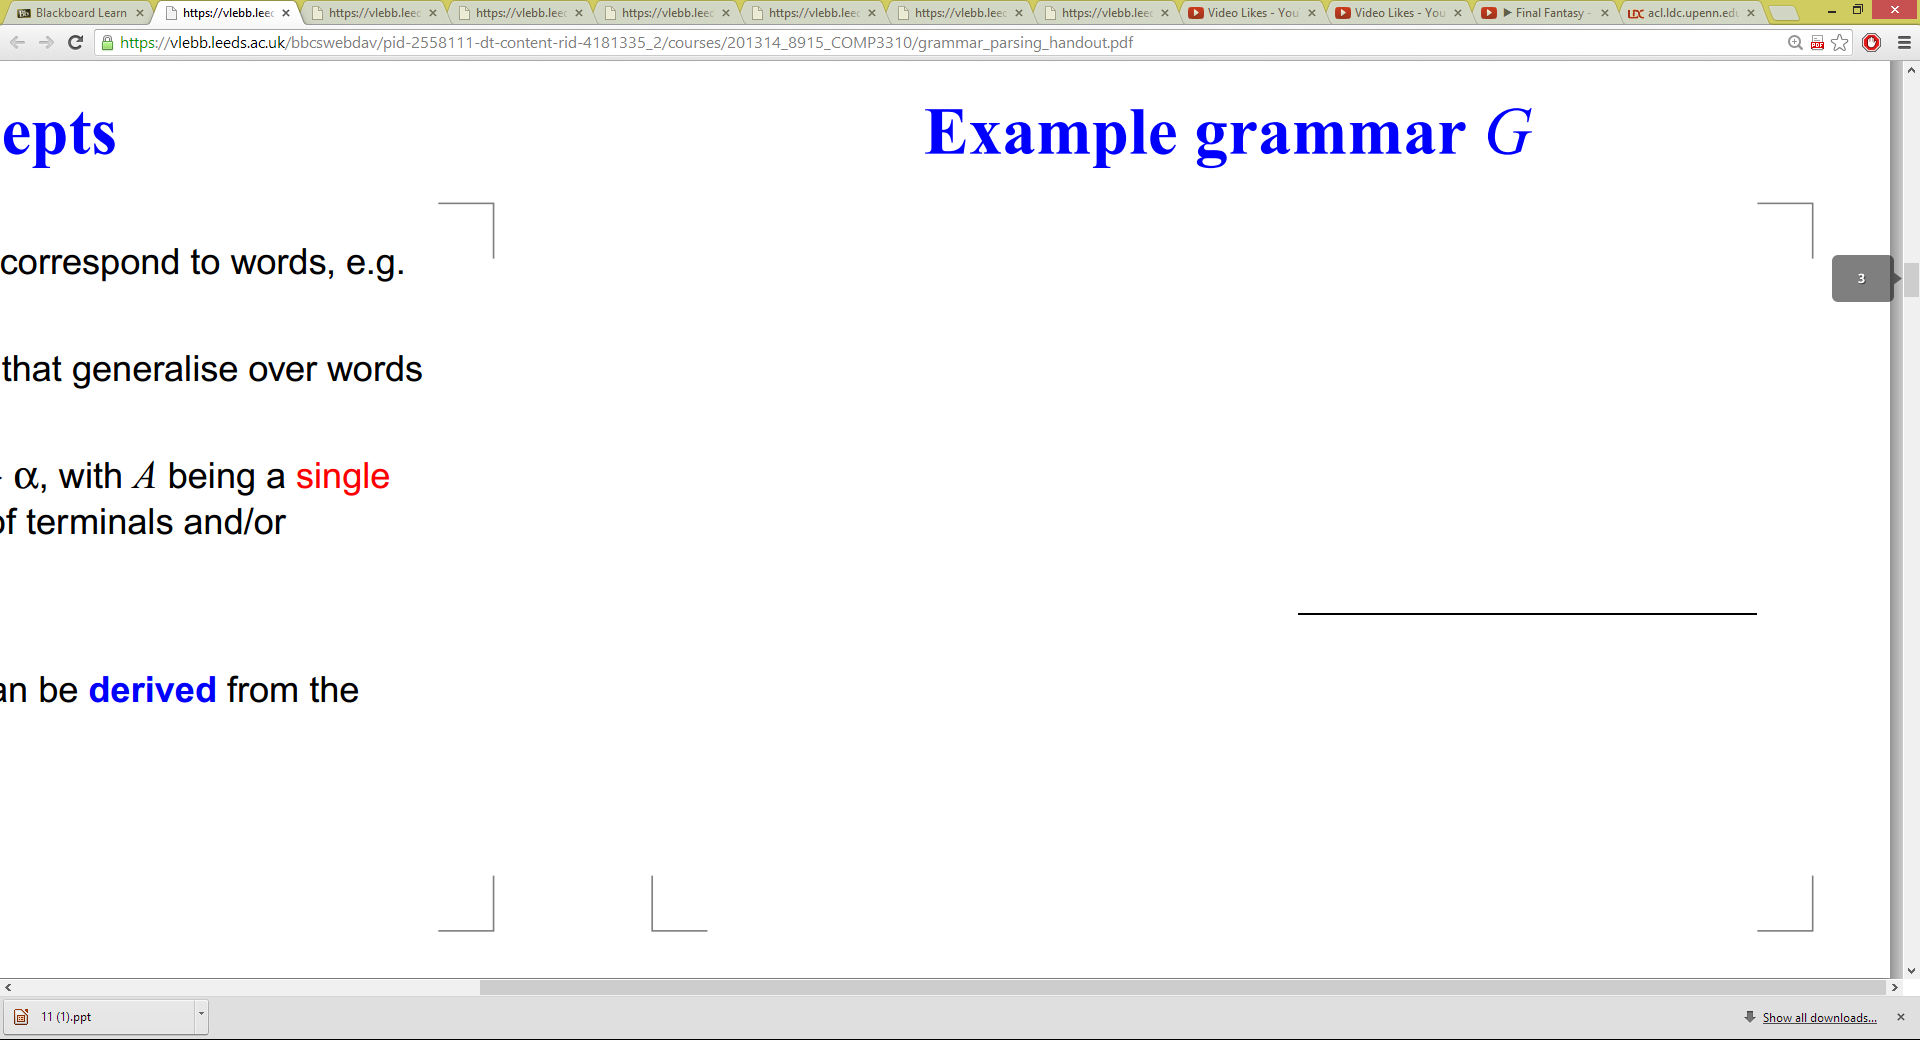
\includegraphics[scale=0.65]{figures/noun-class-hierarchy.png}
	\caption{BNC Probability Model Derived from BNC (rows are first word in bigram)}
	\label{fig:noun-class-hierarchy}
\end{figure}

Table \ref{tab:common-word-classes} lists common word classes that tend to occur in taggers' tagsets, with examples of words.

\begin{table}
	\centering
	\begin{tabular}{|l|l|l|l|}
		\hline
		\textbf{Category} & \textbf{Example} & \textbf{Brown} & \textbf{Penn} \\
		\hline
		Adjective & happy & JJ & JJ \\
		Adverb & often, badly, fast & CD & CD \\
		Determiner & this, each, the & DT & DT \\
		Noun & aircraft & NN & NN \\
		Noun Singular & woman, book & NN & NN \\
		Noun Plural & women, books & NN & NN \\
		Noun Proper Singular & London & NP & NNP \\
		Noun Proper Plural & Australians & NPS & NNPS \\
		Preposition (PP) & on, beneath, beside, over & -- & -- \\
		\hline 
	\end{tabular}
	\caption{Common Word Classes}
	\label{tab:common-word-classes} 
\end{table}

\subsection{Tagsets and Dictionaries}

A \textbf{tagset} is a list of all the possible POS tags in a language. It often encodes morphological categories, like person, number, gender,  case and so on. As an example, the Penn Treebank has 42 tags, while the Brown tag set has 87.

A \textbf{dictionary} maps a \textbf{word} to \textbf{one or more tags}. It is not a one-to-one mapping because words can often have more than tag (as they can used for different grammatical purposes).

Since words can be assigned more than one tag, this means there can be \textbf{ambiguity} in the POS tags. Below is a tagged sentence. "Bush" could be assigned NNP or NN, "fights" could be assigned VBZ or NNS and "press" could be assigned NN or VBD. Since there are \textbf{three} words than can be tagged in \textbf{two} different ways, there are $2^3 = 8$ possible taggings of the sentence.
\begin{quote}
\textit{"Bush fights press"}
\end{quote}
So how do \textbf{resolve} this ambiguity? How do we know which tagging is the right one? We can treat POS tagging as a \textbf{classification task}.

\subsection{POS Tagging as Classification}

Classification tasks are frequent in NLP. Given an observation $o$ and a set of target classes the observation can belong to, determine which target class $o$ belongs to. An an example of this is \textbf{text classification}.

POS tagging as a classification task has the following properties:
\paragraph{}
\begin{tabular}{ll}
	\textbf{Observation:} & a sentence with $n$ words \\
	\textbf{Target Classes:} & all possible tag sequences \\
	\textbf{Restriction on Classes:} & dictionary restricting tags allowed for particular words and sequence must be of length $n$ \\
	\textbf{Knowledge Sources:} & grammatical rules, probabilities from corpora, etc. \\
	\textbf{Knowledge Used:} & lexical (individual word tokens) and syntagmatic (context/surrounding words) \\			
\end{tabular}
\paragraph{}

Two information sources are used in tagging. \textbf{Lexical} information considers the frequencies a particular word is assigned the different tags. For example, \textit{flour/NN vs. flour/VB}. Which is more likely? Perhaps it's the tag that word has been assigned more (based on historical data, like a corpus).

\textbf{Syntagmatic} properties considers sequences of tags surrounding a word. The most likely\textbf{sequence} of tags is chosen. For example, \textit{DD JJ NN vs. DT JJ VB}. Which \textbf{trigram} is more frequent in the training corpus?

A \textbf{unigram tagger} only considers each word by itself, only taking advantage of lexical information. This means it always assigns the word the tag that is most likely, based on the frequency the word has been assigned that tag in a training corpus. Other than that, all taggers use a combination of these two information sources.

\subsection{Markov Model Tagging}

\textbf{Markov models} can be used for POS tag classification, in a similar way $n$-grams can be used for text classification. A Markov model tagger finds the \textbf{most probable tag sequence} $\hat{t_{1,n}}$ for a sequence of words $w_1,...,w_n$ (the sequence could be a sentence, for example). Using Bayes rule, the formula for computing the most probably tag sequence is given in Equation \ref{eq:mm-tag-classification}.

\begin{equation}
\begin{aligned}[b]
	\hat{t_{1,n}} &= max_{t_{1,n}} p(t_{1,n}|w_{1,n}) \\
	&= max_{t_{1,n}} \frac{p(w_{1,n}|t_{1,n})p(t_{1,n})}{p(w_{1,n})} \\
	&= max_{t_{1,n}} p(w_{1,n}|t_{1,n})p(t_{1,n})
\end{aligned}
\label{eq:mm-tag-classification}
\end{equation}

However, this is too difficult to compute, as it requires knowledge of the probabilities of \textit{every single possible} tag and word sequence. Four assumptions are made to simplify this computation:
\begin{enumerate}
	\item \textbf{Markov assumption} (see Section \ref{sec:ngram-modelling}) -- $p(t_i|t_{1,i-1})$
	\item Words are \textbf{independent of each other} --
	$p(w_{1,n}|t_{1,n}) = \prod_{i-1}^n { p(w_i|t_i) }$
	\item Word depends \textbf{only on its tag}, not previous tags -- $p(w_i|t_{1,n}) = p(w_i|ti)$
	\item Time invariance -- $p(t_i|t_{i-1}) = p(t_2|t_1)$
\end{enumerate}

Using these assumptions to simplify the computation gives us the final formula shown in Equation \ref{eq:mm-tag-probability-simplified}. 

\begin{equation}
\begin{aligned}[b]
	p(w_{1,n}|t_{1,n})p(t_{1,n}) &=
	\prod_{i=1}^n { p(w_i|t_{1,n}) p(t_{1,n}) }
	\;\;\;\;\;\;\;\;\;\;\; \text{by assumption (2)} \\
	&= \prod_{i=1}^n { p(w_i|t_{1,n}) \times p(t_n|t_{1,n-1}) \times p(t_{n-1}|t_{1,n-2}) \times ... \times p(t_2|t_1) }
	\;\;\;\;\;\;\;\;\;\;\; \text{by chain rule} \\
	&= \prod_{i=1}^n { p(w_i|t_i) \times p(t_n|t_{n-1}) \times p(t_{n-1}|t_{n-2}) \times ... \times p(t_2|t_1) }
	\;\;\;\;\;\;\;\;\;\;\; \text{by assumption (1) and (3)} \\
	&= \prod_{i=1}^n { \left( p(w_i|t_i) \times p(t_i|t_{i-1}) \right) }
	\;\;\;\;\;\;\;\;\;\;\; \text{rearranging} \\
\end{aligned}
\label{eq:mm-tag-probability-simplified}
\end{equation}
Now the final classification formula, to find the most likely POS tag sequence for a sequence of words, is:
\begin{equation}
	\hat{t_{1,n}} = \max_{t_{1,n}} \prod_{i=1}^n { \left( p(w_i|t_i) \times p(t_i|t_{i-1}) \right) }
\end{equation}

Figure \ref{fig:mm_model} illustrates this simplified Markov model. Some of the probabilities present in the model have been discarded for ease of computation. Only the \textbf{tag-tag bigram probabilities} and \textbf{word-tag unigram probabilities} are considered now.

\begin{figure}[H]
	\centering
	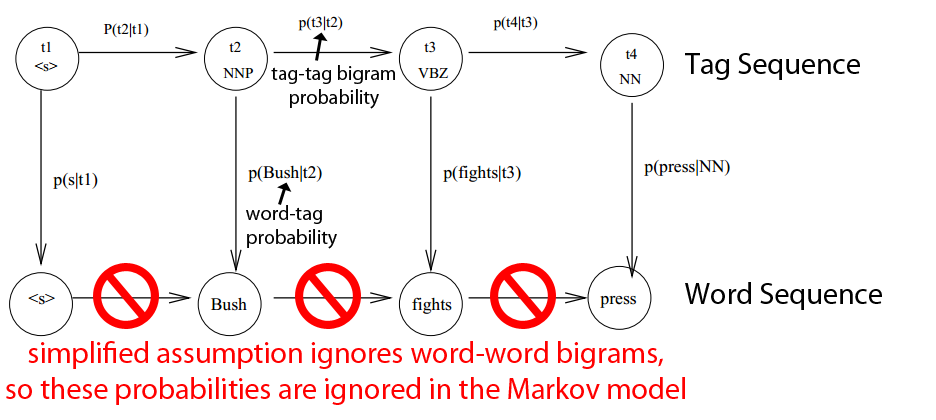
\includegraphics[scale=0.4]{figures/pos-tagging-markov-model.png}
	\caption{Simplified Markov Model for Tag Sequence Prediction}
	\label{fig:mm_model}
\end{figure}

This means we need to built \textbf{two probability models}:
\begin{itemize}
	\item \textbf{Tag-Tag (Bigram) Model} -- A joint probability table which contains the probability of tag $t_i$ following $t_j$, for $i,j \in \lbrace 1, ..., m \rbrace$, where $m$ is the numbers of tags
	\item \textbf{Word-Tag Model} -- Probability of tag $t_i$ being the correct tag for word $w_j$, where $i \in \lbrace 1, ..., m \rbrace$, $j \in \lbrace 1, ..., n \rbrace$, $n$ is the vocabulary size and $m$ is the number of tags
\end{itemize}

Tables \ref{tab:tag-tag-bigram-model} and \ref{tab:word-tag-unigram-model} are examples of tag-tag bigram and word-tag models respectively. These are frequency tables which can be used to compute the probabilities. For example, to compute the probability of a \textbf{noun (NN) following a determiner (DT)}, we do:
\begin{equation}
p(NN|DT) = \frac{f(DT, NN)}{f(DT)} = \frac{48636}{48636 + 19}
\end{equation}
To compute the probability of the word "move" being a noun, we do:
\begin{equation}
p(move|NN) = \frac{f(NN,move}{f(NN)}) = \frac{36}{81036}
\end{equation}
Note that some words/tokens \textbf{always} have the same tag, so the probability is 1. This is the case with "." and "is", which always have the PERIOD and VBZ tags respectively.

\paragraph{\textbf{NOTE: }} To compute these probabilities, the joint probabilities are not the only thing required. The \textbf{singular probabilities for tags} (e.g. $p(DT)$) must be computed. This is done by filling in the "Total" row and column in Table \ref{tab:tag-tag-bigram-model}.
\paragraph{}

\begin{table}
	\centering
	\begin{tabular}{r|lllllll}
		\textbf{First Tag $\lor$} & DT & VBZ & IN & NN & VB & PERIOD & \textbf{Total} \\
		\hline
		DT & 0 & 0 & 0 & 48636 & 0 & 19 & - \\
		VBZ & 1973 & 0 & 426 & 187 & 0 & 38 & - \\
		IN & 43322 & 0 & 1325 & 17314 & 0 & 185 & - \\
		NN & 1067 & 3720 & 42470 & 11773 & 614 & 21392 & - \\
		VB & 6072 & 42 & 2758 & 1476 & 129 & 1522 & - \\
		PERIOD & 8016 & 75 & 4656 & 1329 & 954 & 0 & - \\
		\textbf{Total} & - & - & - & - & - & - & - \\
	\end{tabular}
	\caption{Tag-Tag Bigram Model from a Tagged Training Corpus}
	\label{tab:tag-tag-bigram-model}
\end{table}

\begin{table}
	\centering
	\begin{tabular}{r|llllll}
		\textbf{Words $\lor$} & DT & VBZ & IN & NN & VB & PERIOD \\
		\hline
		bear & 0 & 0 & 0 & 10 & 43 & 0 \\
		is & 0 & 10065 & 0 & 0 & 0 & 0 \\
		move & 0 & 0 & 0 & 36 & 133 & 0 \\
		on & 0 & 0 & 5484 & 0 & 0 & 0 \\
		the & 69016 & 0 & 0 & 0 & 0 & 0 \\
		. & 0 & 0 & 0 & 0 & 0 & 48809 \\
	\end{tabular}
	\caption{Word-Tag Unigram Model from a Tagged Training Corpus}
	\label{tab:word-tag-unigram-model}
\end{table}

\subsubsection{Advantages/Disadvantages}

\textbf{Advantages}:
\begin{itemize}
	\item $k$-best tagging is possible, which is powerful tagging technique often necessary for parsing decisions
	\item Based purely on statistics, so \textbf{prior linguistic knowledge} does not need to be encoded, making the technique \textbf{language-agnostic}
\end{itemize}

\textbf{Disdvantages}:
\begin{itemize}
	\item It makes crude assumptions, so it may not model the real language accurately enough
	\item Only deals with \textbf{very short distance dependencies} between words (due to the fact that the $n$-gram model is being used)
	\item Tags are never conditioned on words 
	\item \textbf{Unintuitive}, can be hard to understand
\end{itemize}

\subsection{Transformation-Based Tagging}

Markov models only identifies a \textbf{small range} of regularities present in natural language. \textbf{Transformation-based tagging} encodes more \textbf{complex} interdependencies between words and tags. It does this by learning \textbf{intuitive} rules from a training corpus. Unlike Markov model tagging, this \textbf{exploits prior linguistic knowledge} of a language, through the use of templates (described later). 

Transformation-based learnings takes \textbf{two inputs}:
\begin{enumerate}
	\item tagged training corpus and word-tag dictionary
	\item \textbf{templates} that encode \textit{specifications} for admissible transformations (e.g. \texttt{Change Tag1 to Tag2 if the preceding word is tagged Tag3})
\end{enumerate}
After receiving these, a learning algorithm learns \textbf{transformation instantiations} from the tagged training corpus. These are instantiations of the transformation templates given to it. The \textbf{output} of the learning algorithm is a \textbf{ranked list of transformation instantiations} that can be applied (in order of rank) to another unseen, untagged corpus. The idea is that this ranked list of transformations produces accurate taggings in unseen texts.

\textbf{Templates} specify general, admissible transformations. These transformations must always be legal and never break down the tagf sequence. There are three major types of templates -- \textbf{tag-driven}, \textbf{word-driven} and \textbf{morphology-driven}.

Examples of tag-driven templates include: \texttt{Change Tag1 to Tag2 if}
\begin{itemize}
	\item \texttt{The preceding/following word is tagged Tag3}
	\item \texttt{The word two before/after is tagged Tag3}
	\item \texttt{One of the $n$ preceding/following words is tagged Tag 3}
	\item \texttt{The preceding word is tagged Tag3 and the following word is tagged Tag4}
	\item \texttt{The preceding/following word is tagged Tag3 and the word two before (after) is tagged Tag4}
\end{itemize}

Example of a word-drive template: \texttt{Change Tag1 to Tag2 if the previous word is W3}

Example of a morphology-drive template: \texttt{Change Tag1 to Tag2 if the word ends with Suffix1}

How does the algorithm \textbf{learn} which transformation rules work best? Given a training corpus $T$, the following \textbf{learning algorithm} is applied:
\begin{enumerate}
	\item \textbf{Assume you don't know} the correct tagging sequence for $T$
	\item Tag each word in $T$  with its \textbf{most frequent tag} (learnt from training corpus). For example, $move \implies VB$.
	\item Consider \text{all} possible transformations and apply the one that improves tagging accuracy the most (accuracy measure derived from $T$). This is a form of \textbf{greedy search}, which selects a single template instantiation every iteration (e.g. \texttt{Change VB tp NN if the precediing word is tagged DT}).
	\item Retag $T$ applying that rule
	\item Go back to 3 and repeat (baseline corpus accuracy $T$ is now the retagged one from step 4). This is done \textbf{until significant improvements are reached} (could use threshold as stopping criterion).
	\item Return all learnt rules \textbf{in order}
\end{enumerate}
This greedy algorithm is iterative and will continuously run until terminated by its stopping criteria (e.g. converges to best accuracy it can find -- maxima). Figure \ref{fig:transformed-based-tagging} illustrates the iterative process. Notice how it builds upon the previous rules at each iteration, and how the initial tagging is performed by a \textbf{baseline tagger} (e.g. unigram tagger).

\begin{figure}
	\centering
	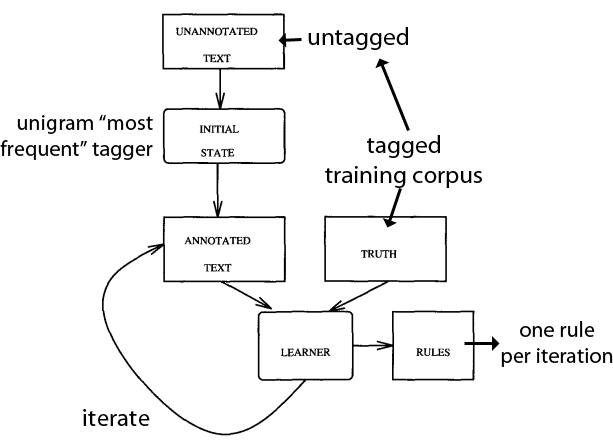
\includegraphics[scale=0.4]{figures/transformed-based-tagger.png}
	\caption{Transformation-Based Tagging Learnign Algorithm}
	\label{fig:transformed-based-tagging}
\end{figure}

Consider the example corpus in Table \ref{tab:transformation-tagger-example1}, whose approximated tags have been initialised with the \textbf{most frequent tag}. The entries in \textbf{bold} have not been tagged correctly in the approximation. The first iteration of the algorithm finds \texttt{Change VB to NN if previous tag is DT} to be the rule which results in the best accuracy, so it saves that rule and retags the corpus. This is shown in  Table \ref{tab:transformation-tagger-example2}.

A second iteration finds \texttt{Chnage NN to VB if previous tag is TO} to be the best trasformation next. The rule is saved and the corpus is retagged to achieve the approximation in Table \ref{tab:transformation-tagger-example3}. Note how we have achieved 100\% accuracy now, so the algorithm terminates and returns the ordered list of rules that were found:
\begin{enumerate}
	\item \texttt{Change VB to NN if previous tag is DT}
	\item \texttt{Change NN to VB if previous tag is TO}
\end{enumerate}

\begin{table}[H]
	\centering
	\begin{tabular}{|l|l|}
		\hline
		\textbf{Training Corpus} & \textbf{Approximation \#0} \\
		\hline
		The/DT & The/DT \\
		bear/NN & \textbf{bear/VB} \\
		is/VBZ & is/VBZ \\
		on/IN & on/IN \\
		the/DT & the/DT \\
		move/NN & \textbf{move/VB} \\
		to/TO & to/TO \\
		race/VB & \textbf{race/NN} \\
		there/RB & there/RB \\
		\hline
	\end{tabular}
	\caption{Approximation using initial most frequent tagger}
	\label{tab:transformation-tagger-example1}
\end{table}

\begin{table}[H]
	\centering
	\begin{tabular}{|l|l|}
		\hline
		\textbf{Training Corpus} & \textbf{Approximation \#1} \\
		\hline
		The/DT & The/DT \\
		bear/NN & bear/NN \\
		is/VBZ & is/VBZ \\
		on/IN & on/IN \\
		the/DT & the/DT \\
		move/NN & move/NN \\
		to/TO & to/TO \\
		race/VB & \textbf{race/NN} \\
		there/RB & there/RB \\
		\hline
	\end{tabular}
	\caption{Approximation using one found rule}
	\label{tab:transformation-tagger-example2}
\end{table}

\begin{table}[H]
	\centering
	\begin{tabular}{|l|l|}
		\hline
		\textbf{Training Corpus} & \textbf{Approximation \#1} \\
		\hline
		The/DT & The/DT \\
		bear/NN & bear/NN \\
		is/VBZ & is/VBZ \\
		on/IN & on/IN \\
		the/DT & the/DT \\
		move/NN & move/NN \\
		to/TO & to/TO \\
		race/VB & race/VB \\
		there/RB & there/RB \\
		\hline
	\end{tabular}
	\caption{Final approximation using first and second found rules}
	\label{tab:transformation-tagger-example3}
\end{table}


\subsubsection{Advantages/Disadvantages}

\textbf{Advantages:}
\begin{itemize}
	\item Uses wider context and \textbf{following} context (not just previous), enabling it to learn more complex patterns
	\item Can be expanded to word-driven templates for greater detail
	\item Can be expanded to morphology-drive templates, which is \textbf{great for unknown words}
	\item Learn rules are \textbf{easy to understand} by humans, they're \textbf{intuitive}
\end{itemize}

\textbf{Disadvantages:}
\begin{itemize}
	\item Hard to use for $k$-best tagging, which is important for parsing grammar
	\item Uses pre-encoded linguistic knowledge, meaning that for each language youneed to specify new templates
\end{itemize}

\subsection{Evaluation and Performance Issues}

Taggers can be \textbf{evaluated} by simply measuring the \textbf{accuracy} (\%) of the tagger when used on (unseen) test corpora. 11,5\% of \textbf{word types} have more than one tag, which makes tagging seem like an easy problem. However, 40\% of \textbf{tokens} have more than one tag; that is, almost the tags of almost half of all text is ambiguous. Therefore, tagging is no easy task.

The \textbf{upper bound} can be decided by having humans tag corpora and measuring their accuracy. Currently, there exist taggers which can achieve \textbf{95\% to 97\% accuracy}. A sensible \textbf{lower bound} is \textbf{90\%}, since that's the accuracy some unigram "most frequent" taggers have achieved.

\textbf{Tagging performance} (accuracy) depends on many variables, such as:
\begin{itemize}
	\item corpus size (amount of training data)
	\item genre and formality of training and test data (do they differ?)
	\item mistakes in pre-tagged training corpora (or mistakes in the actual \textit{text} which result in incorrect grammar)
	\item number of unknown words in text (taggers often struggle with unknown words)
\end{itemize}

\section{Grammar and Parsing}

In order to get even more information on text, we can make use of grammar and parsing to group words into a hierarchy that describes the true meaning of the text. 

\subsection{Constituents}

A \textbf{constituent} is a group of words that \textbf{behave as a single unit}. They can be thought of as \textbf{phrases}, which can be nested within each other. These are different \textbf{types} of constituents/phrases, each of which are composed of different things. Below is an example o fa sentence broken down into its constituents, with each constituent labelled with its type:
\begin{quote}
	$[_{NP}$She] saw $[_{NP}$him] $[_{PP}$on Friday]
\end{quote}
"on Friday" is an individual constituent/phrase. This particular one is a \textbf{prepositional phrase}, as indicated by the $PP$. Constituents can also be \textbf{nested} within each other:
\begin{quote}
	$[_{NP}$old men $[_{PP}$with $[_{NP}$hats]]]
\end{quote}
This nesting expresses \textbf{attachment}, making one constituent related to another. When combined, constituents create a \textbf{whole new}, valid constituent that has a different meaning. The order/way constituents are composed does change the meaning of the final sentence.

How do you know if a group of words are \textit{actually} a constituent? They are if they express \textbf{movability}. If you think a group of words is a constituent, try \textbf{breaking the constituent up}, by moving some of the words inside it to another place in the sentence. If the sentence \textit{or} the new constituent does not make sense, then it's likely they are \textbf{not} a constituent. Similarly, if you think you have one, try moving the \textit{entire} group of words \textbf{together}, to another place in the sentence. If both the constituent and sentence still makes sense, then you probably have a constituent. Consider the following example:
\begin{quote}
	$[_{NP}$She] saw $[_{NP}$him] $[_{PP}$on Friday seventeenth]. \textbf{VALID} \\
	$[_{PP}$on Friday seventeenth], $[_{NP}$She] saw $[_{NP}$him]. \textbf{VALID} \\
	$[_{PP}$on Friday], $[_{NP}$She] saw $[_{NP}$him] seventeenth \textbf{INVALID} \\
\end{quote}
The first line is the original sentence, the second is a sentence formed by moving the \textbf{entire} constituent "on Friday seventeenth". This is still a valid sentence. The third sentence was formed by moving \textbf{part} of "on Friday seventeenth" ("on Friday"). Notice how the third sentence is not grammatically correct and does not make sense. This is a strong indicator that "on Friday seventeenth"  is a valid constituent (they make sense together, but not on their own).

How do you \textbf{determine} if two constituents, $A$ and $B$, are the \textbf{same type}? You check if they have the \textbf{substitution} property. If you can \textbf{swap} $A$'s and $B$'s position in the text, and the resulting sentence is grammatically correct, then you have the \textbf{same type of constituent}.

\subsection{Limitations with $n$-grams and Regular Expressions}

Constituents are \textbf{different} from $n$-grams. $n$-grams can stop \textit{within} a constituent, or \textit{cross} constituent boundaries to be inside more than one. Additionally, $n$-grams do not express \textbf{movability} or\textbf{long-distance dependencies}. Due to the nested nature of constituents, long distance dependencies can be found. This is also possible with $n$-grams if $n$ is large, but due to data sparseness and how computationally/memory intensive it would be, it's just not feasible.

Therefore, $n$-grams fail to express entities and dependencies \textit{between} entities \textbf{in full}.

\textbf{Regular expressions} are able to parse \textbf{regular} languages. However, they cannot fully parse hierarchical languages. \textbf{Context-free grammars}, such as English, French and HTML, can be hierarchical.  Consider the following example:
\begin{quote}
	The cat and the dog with the hat love the cow
\end{quote}
Here, the cat loves the cow. However, since regular expressions cannot express \textbf{attachment} (nesting), it won't detect that "the dog with the hat" is nested with the cat and that \textit{both} the cat and the dog love the cow. Therefore, regular expressions \textbf{cannot} be used to fully express entities and their dependencies in natural languages either, as \textbf{recursion/nesting} accounts for a large chunk of the complexity in human language.

\subsection{Grammar}

A \textbf{grammar} describes the \textbf{rules} of bracketing for a language, as well as the \textbf{regularities} of how the constituents are grouped together and attached to each other (what's nested in what).

A \textbf{rule} is defined by a left-hand side (LHS) and a right-hand side (RHS). The LHS contains a type of phrase/constituent and the RHS is what the constituent contains. For example:
\begin{quote}
	$NNS \rightarrow \lbrace$ women, men, tables $\rbrace$ \\
	$NP \rightarrow AT\;NNS$
\end{quote}
defines a \textbf{lexicon} of words and their \textbf{parts of speech}. It states that the $NP$ constituent type can contain $AT$ and $NNS$ constituents/words, and that the words "women", "men" and "tables" have the POS tag $NNS$.

A grammar consists of:
\begin{itemize}
	\item \textbf{Terminal Symbols} -- symbols that correspond to groups of words (e.g. "table", "apple", "laughing")
	\item \textbf{Non-Terminal Symbols} -- symbols that \textbf{generalise} over words or other non-terminals (e.g. $NP$). This is how \textbf{recursion} and nesting are introduced
	\item \textbf{Context-Free Grammar Rule} $A \rightarrow \alpha$ -- where $A$ is a \textbf{single non-terminal} and $\alpha$ is a \textbf{sequence} of terminals and/or non-terminals
	\item \textbf{Start Symbol} $S$ -- Where the generation of string using the grammar starts
	\item \textbf{Language} $L(G$ -- a set containing \text{all strings} that can be \textbf{derived} from the start symbol via the rules
\end{itemize}

An example grammar $G$ is shown in Figure \ref{fig:example-grammar}. The top half defines the \textbf{rules} of the grammar and the bottom half defines the \textbf{lexicon} (vocabulary).

\begin{figure}
	\centering
	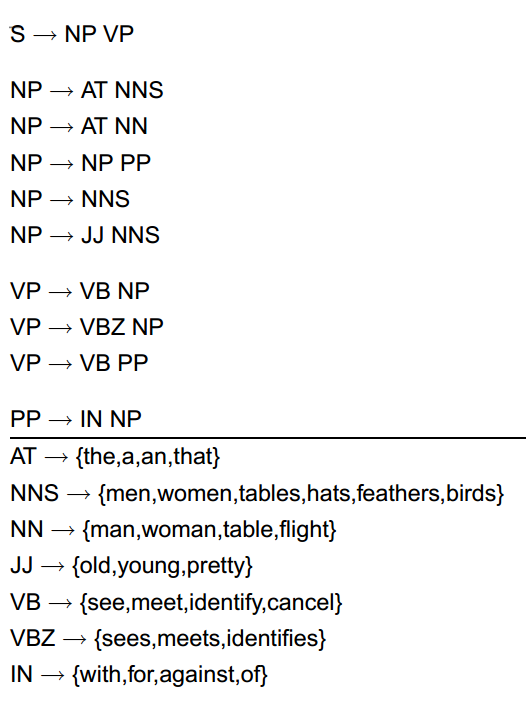
\includegraphics[scale=0.4]{figures/example-grammar.png}
	\caption{Example Context Free Grammar $G$}
	\label{fig:example-grammar}
\end{figure}

An example of deriving a sentence using the production rules of the grammar $G$ in Figure \ref{fig:example-grammar} is shown in Equation \ref{eq:example-sentence-derivation}. Both Equation \ref{eq:example-sentence-derivation-bracketing} and Figure \ref{fig:example-sentence-derivation} illustrate the \textbf{nested hierarchy} of terminals that produced the sentence (the former with \textbf{bracketing} and the latter with a \textbf{syntax tree}).

\begin{equation}
\begin{aligned}[b]
	S &\rightarrow NP\; VP \\
	&\rightarrow AT \; NNS \; VB \; NP \\
	&\rightarrow AT \; NNS \; VB \; JJ \; NNS \\
	&\rightarrow \text{The men see old women}
	\label{eq:example-sentence-derivation}
\end{aligned}
\end{equation}

\begin{equation}
	[_{S}[_{NP}[_{AT}the] [_{NNS}men]] [_{VP}[_{VB}see] [_{NP}[_{JJ}old] [_{NNS}women]]]]
	\label{eq:example-sentence-derivation-bracketing}
\end{equation}

\begin{figure}
	\centering
	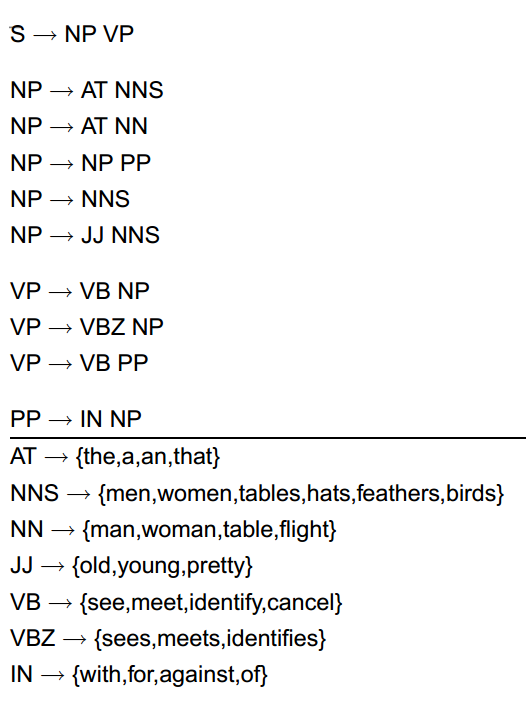
\includegraphics[scale=0.4]{figures/example-grammar.png}
	\caption{Parse Tree for Sentence \textit{"The men see old women"}}
	\label{fig:example-sentence-derivation}
\end{figure}

Consider the following sentences. Which are grammatical (valid) under grammar $G$?
\begin{enumerate}
	\item \textbf{(VALID)} -- The men with the hats with the feathers see old women
	\item \textbf{(INVALID)} -- The children see old women
	\item \textbf{(VALID)}  -- Old women sees old men
	\item \textbf{(INVALID)} -- See old women!
\end{enumerate}
Sentence 2 is invalid because it contains a word \textbf{not specified in the grammar's lexicon} ("children").  Sentence 4 is invalid because there is \textbf{no rule} which states a verb can be at the start of sentence (see is part of the terminal class "VB")

\subsubsection{Limitations}

\textbf{Agreement} is when  the number, case or gender of two constituents must agree, or match. For example, "the dogs sees the bone". "sees" is only used for singular nouns -- the correct word is "see". However, context-free grammars do not take this into consideration. There are two ways to solve this:
\begin{itemize}
	\item Use a context-sensitive language
	\item Use \textbf{constraint-based formalism}. An example of a rule with constrains is "$S \rightarrow NP VP$, only if the number of $NP$ is equal to the number of $VP$".
\end{itemize}

While defining the syntax and lexicon of a grammar (e.g. for English) is useful, what happens when you have a sentence that can be parsed in multiple different ways (i.e. \textbf{ambiguity})? The parse that makes sense depends on the words actually being used. In other words, the \textbf{semantics} of the words and the overall meaning of the sentence can affect parsing decisions.
\begin{quote}
	I eat the cake with a spoon. \\
	I eat $[_{NP}$the cake with a spoon.]
\end{quote}
The above parse would mean that the person speaking is eating a cake, and that the cake owns/is holding a spoon. The highlights that syntax is \textbf{not clearly separated from semantics}.

The big question in all this is: are human languages context-free? Are context-free grammars able to describe all language phenomena? Or do you only need rules like $A \rightarrow \alpha$? \textbf{English} seems to be context free, but others may not be. For example, \textbf{Swiss German} is \textit{not}, it is \textbf{context sensitive}. Whether or not a language is truly context-free must be considered before trying to construct a grammar to parse it.

\subsection{Parsing}

\textbf{Parsing} assigns a \textbf{syntactic structure} to a sentence, such as a CFG tree. A \textbf{parse} is a tree (of constituents) constructed from a sentence. Parsing has many applications, such as:
\begin{itemize}
	\item Grammar checking (e.g. compiling programming languages)
	\item Intermediate stage to full semantic analysis
	\item Machine translation, information extraction, question asking (parsing gives groupings of words, which can be used to get semantics/information on text's content)
\end{itemize}

\textbf{Automatic parsing} searches through \textbf{all possible parse trees} to find the correct tree, in a brute-force manner. There are two major types of parsing:
\begin{itemize}
	\item \textbf{Top-Down Parsing} -- Search for a parse tree that fits the input text by trying to build \textbf{from the root} $S$ to the leaves (tokens in text)
	\item \textbf{Bottom-Up Parsing} -- Build a parse tree \textbf{from the leaves} (tokens), moving upwards to the root
\end{itemize}
Parsers are often a combination of the two approaches.

Figure \ref{fig:top-down-parsing} shows an example of using the standard \textbf{brute force top-down search algorithm} to find the correct parse tree for the sentence \textit{"See the women"}. It also shows what the final parse tree looks like. Notice how the parser may have to backtrack one or more times it finds invalid parse trees.

\begin{figure}
	\centering
	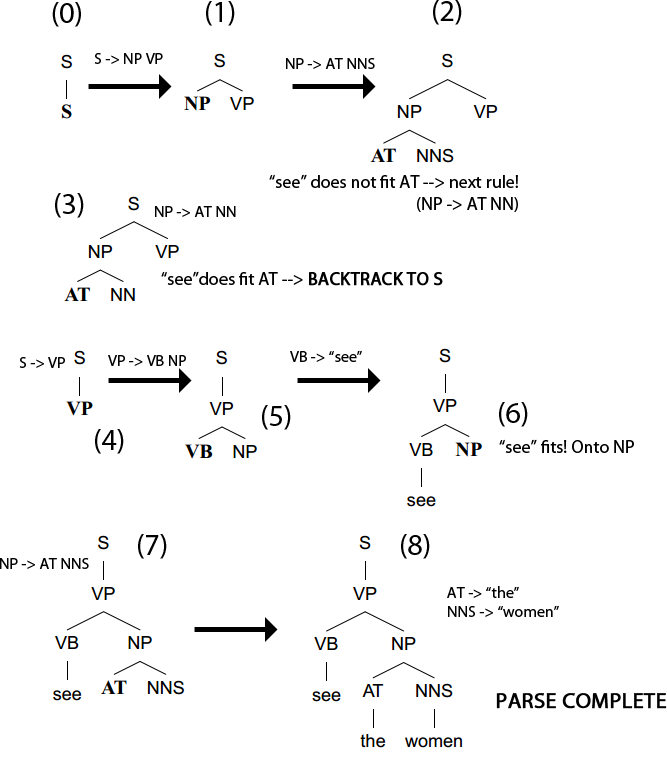
\includegraphics[scale=0.4]{figures/top-down-parsing-example.png}
	\caption{Example of Top-Down DFS Parsing to Find Valid Parse for Sentence \textit{"see the women"}}
	\label{fig:top-down-parsing}
\end{figure}

\paragraph{\textbf{NOTE: }} Typically, these search algorithms choose \textbf{production rules} to apply in the \textbf{same order they are specified in the grammar}. Additionally, children of a parse tree are evaluated from left-to-right (left-most node of search tree is expanded first). 
\paragraph{}

This search algorithm is essentially \textbf{depth-first search (DFS)}. DFS systemically explores the search space by concentrating on one state at a time. When there is an \textbf{inconsistency} between the current tree and the sentence, the algorithm \textbf{backtracks} to the \textbf{most recently generated unexplored} tree (most recent unexplored node).

\subsubsection{Limitations}

The top-down DFS search algorithm uses rules that we \textit{know} are invalid due to POS (part-of-speech) tagging constraints. For example, "the" is \textit{always} a determiner, but the brute force search will even consider it to be other tags (e.g. nouns or verbs). This causes lots of backtracking and drastically slows down parsing times.

One solution to this is to \textbf{combine} the top-down approach with \textbf{bottom-up filtering}. You start the top-down and bottom-up parses \textbf{at the same time}. Any trees/subtrees found to be invalid on the bottom-up search will be \textbf{filtered} from the top-down approach, so it won't even consider them.

Another problem with parsing is \textbf{infinte recursion}. If there is even one recursive production rule in the grammar, then DFS could get stuck in an infinite loop, where it is constantly applying the same production rule over and over. This is shown in Figure \ref{fig:infinite-recursion} for the grammar:
\begin{equation}
\begin{aligned}[b]
S \rightarrow NP \\
NP \rightarrow NP PP
\end{aligned}
\end{equation}

\begin{figure}
	\centering
	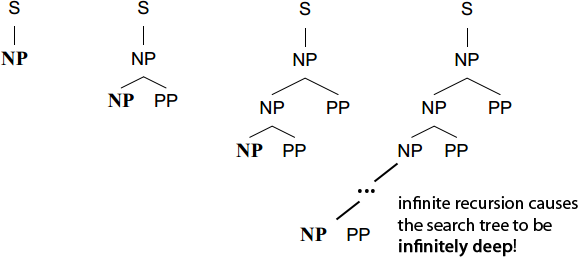
\includegraphics[scale=0.4]{figures/infinite-recursion.png}
	\caption{Example of Infinite Recursion Caused by Production Rule NP -> NP PP}
	\label{fig:infinite-recursion}
\end{figure}

Top-down DFS recomputes the same parse trees many times. Consider the two parse trees the search generated at different states in Figure \ref{fig:effort-duplication}. Notice how the tree A is a subtree of a node in tree B? DFS will compute the entire sub-tree \textbf{again}, which results in a \textbf{duplication of effort}.

\begin{figure}
	\centering
	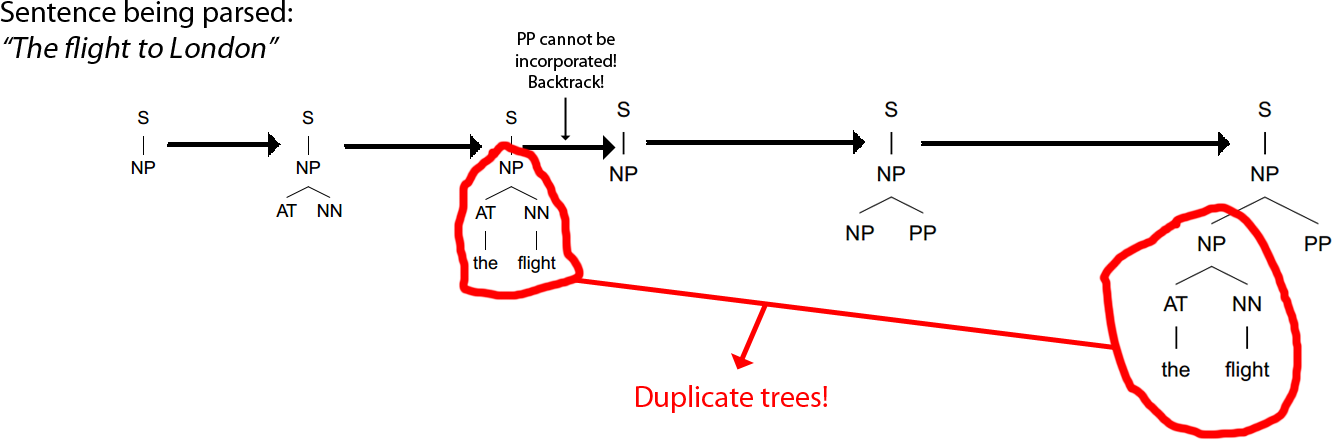
\includegraphics[scale=0.3]{figures/parsing-effort-duplication.png}
	\caption{Effort Duplication Using Top-Down DFS Parser}
	\label{fig:effort-duplication}
\end{figure}

\textbf{Chart parsing} reduces the overall computation time by storing constituents or trees in a \textbf{table/chart}. When expanding a node, the table can be looked up to see if a tree already exists for that expansion from a previous expansion (worse case complexity for this is $n^3$).

\subsection{Global Ambiguity}

Consider the sentence:
\begin{quote}
	\textit{The students see old men with the binoculars}
\end{quote}
Figure \ref{fig:global-ambiguity} shows how there are \textbf{multiple ways} to \textit{correctly} parse the sentence. That is, multiple valid bracketings or trees can be produced. This is \textbf{syntactic ambiguity}, where a sentence/constituent has more than one parse because of ambiguity after how \textbf{syntactic constituents combine}. This is not ambiguity causes by words; it's caused by how the words are syntactically built up into a sentence using the grammar's rules.

\begin{figure}
	\centering
	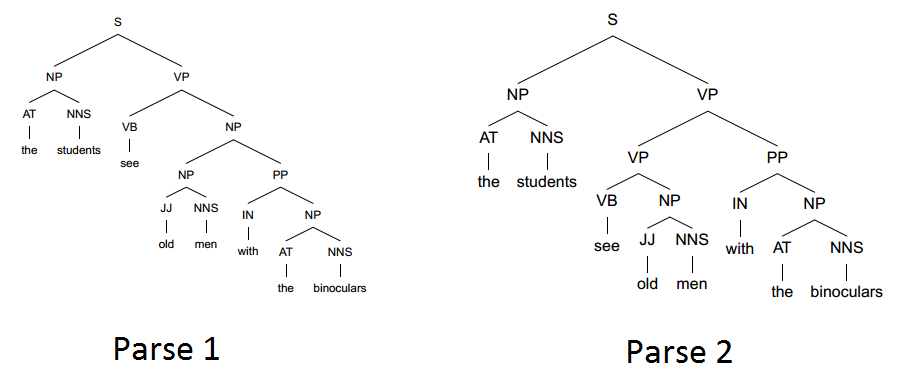
\includegraphics[scale=0.6]{figures/multiple-parses-example.png}
	\caption{Two Valid Parses for Same Sentence \textit{"the students see old men with the binoculars"}}
	\label{fig:global-ambiguity}
\end{figure}

The main types of ambiguity are:
\begin{itemize}
	\item \textbf{Categorical/POS Ambiguity} -- One word can have several different parts of speech tagging. For example, "throw" can be a verb or a noun (to "throw" something, or a light cover for furniture)
	\item \textbf{Lexical/Sense Ambiguity} -- When a word has a single syntactic category (same POS tag), but has \textbf{at least two different meanings}. For example, "port" can mean a place for ships to dock or the alcoholic drink.
	\item \textbf{Syntactic Ambiguity} -- A sentence/constituent having \textbf{more than one parse because} of ambiguity about how syntactic constituents combine
\end{itemize}
Categorical ambiguity often leads to syntactic ambiguity.

Syntactic ambiguity results in \textbf{exponential explosion} (it follows the Catalan numbers), which means the number of possible different parses increases exponentially. This can cause serious issues for parsing -- if there's an exponential number of different parses, how can evaluate all the different parses to find the right ne?

\textbf{Global ambiguity} refers to this situation where there is more than one parse for the \textbf{whole sentence}. How can you compute the correct parsing for a sentence when there is such ambiguity? There are are two ways:
\begin{itemize}
	\item return all parse
	\item \textbf{make a decision} and return a single preferred parse (like humans do)
\end{itemize}

\subsubsection{Probabilistic Context Free Grammars}

So how do you make a decision and select a preferred parse to handle global ambiguity? One way is \textbf{probabilistic context free grammars (PCFG)}. These grammars contain context-free rules that are \textbf{annotated with probabilities}. Probabilities of all rules with the \textbf{same left hand side} sum to one. The \textbf{probability of a parse} is then the \textbf{product} of the probabilities of all rules applied in the parse. Figure \ref{fig:probabilistic-grammar} shows an example of a probabilistic context-free grammar, which is a list of production rules and their probabilities. The probabilities of $VP \rightarrow VB\;NP$ and $VP \rightarrow VP\;PP$ sum to one, as they are the only two production rules with $VP$ as the left hand side.

\paragraph{\textbf{NOTE: }} Notice how the POS tags that words can have (terminals) have probabilities too, such as $IN \rightarrow \text{with}$ having a probability of 1.

\begin{figure}
	\centering
	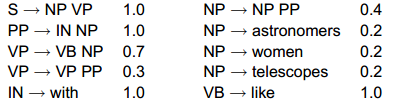
\includegraphics[scale=0.7]{figures/probabilistic-grammar-example.png}
	\caption{Example Probabilistic Context-Free Grammar}
	\label{fig:probabilistic-grammar}
\end{figure}

Let $t_1$ and $t_2$ be two different (valid) parses for the sentence \textit{"astronomers like women with telescopes"}, using the probabilistic grammar from Figure \ref{fig:probabilistic-grammar}. Figure \ref{fig:example-probabilistic-parses} shows the parse trees for $t_1$ and $t_2$. The probabilities of both parses being the correct parsing for the sentence is computing by multiplying all the individual parses , like so:
\begin{equation}
\begin{aligned}[b]
	P(t_1) &= P(S \rightarrow NP VP) \times P(NP \rightarrow \text{astronomers}) \times ... \times P(NP \rightarrow \text{telescopes})  \\
	 &= 1.0 \times 0.2 \times 0.7 \times 1.0 \times 0.4 \times 0.2 \times 1.0 \times 1.0 \times 0.2 \\
	&= 0.0024 \\
\end{aligned}
\end{equation}
\begin{equation}
\begin{aligned}[b]
	P(t_2) &= P(S \rightarrow NP VP) \times P(NP \rightarrow \text{astronomers}) \times ... \times P(NP \rightarrow \text{telescopes})  \\
	 &= 1.0 \times 0.2 \times 0.3 \times 0.7 \times 1.0 \times 1.0 \times 0.2 \times 1.0 \times 0.2 \\
	&= 0.00168 \\
\end{aligned}
\end{equation}
$P(t_1) > P(t_2)$, so we choose $t_1$ as the parse for the sentence \textit{"astronomers like women with telescopes"}.

\begin{figure}
	\centering
	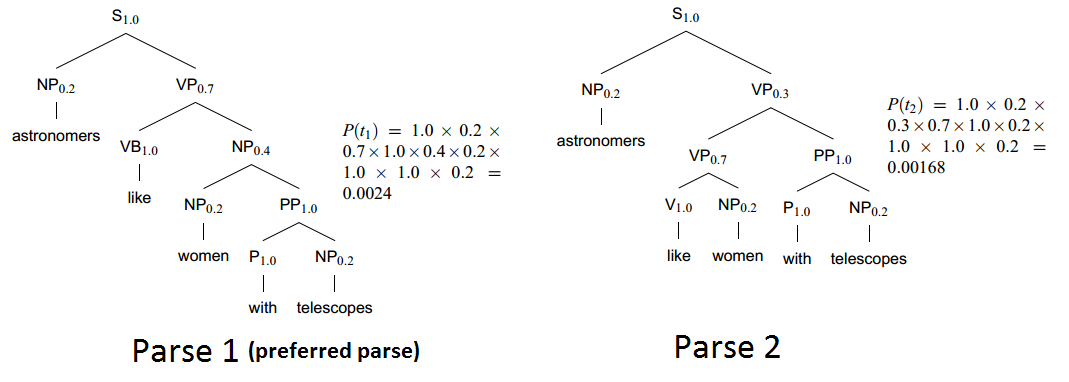
\includegraphics[scale=0.55]{figures/example-probabilistic-parses.png}
	\caption{Probabilistic Parsing of Sentence \textit{"astronomers like women with telescopes"} to Find a Single Preferred Parse}
	\label{fig:example-probabilistic-parses}
\end{figure}

This approach expresses preferences for \textbf{local attachment}, which means \textbf{larger groupings of words}. Another way of thinking about it is that it expresses preference for \textbf{wide, shallow} trees. This is because every non-terminal's probability is multiplied with the final probability, which will \textit{reduce} the overall probability of the parse. More non-terminals (smaller groupings and a deeper tree) typically mean more probabilities.

\subsubsection{Frame Preferences}

$t_1$ states that the women have the telescopes, whereas $t_2$ states that the men have the teleschopes. Suppose "like" was replaced with "observe", to make the sentence \textit{"astronomers observe women with telescopes"}. The correct parse is clearly $t_2$, as telescopes are used to observe things . However, using the described approach to determine the most likely parse would still prefer $t_1$. The method does not take the \textbf{semantics}, or meaning, carried by a word.

PCFG does not account for \textbf{lexical preferences}. Verbs can have several \textbf{subcategorisation frames} (phrases it selects for), are are the non-terminals/terminals that appear after the word. Some frames are preferred (i.e. are more likely) over others. Table \ref{tab:frame-examples} shows the subcategorisation frames of the verb \textit{keep}. \textbf{Frame probabilities} tells us how likely each of these frames (for that particular verb) is. This information can be combined with \textbf{construction probabilities} generated by a PCFG (probabilities discussed earlier).

How can frame probabilities be computed? One method is to use a corpus that's annotated with \textbf{parse tree structures} (e.g. Penn Treebank) to estimate frame probabilities of each verb from the corpus. For a \textbf{usable and accurate} probability model, \textbf{very large corpora} are required. Due to the complexity of having humans manually parse sentences, this is very difficult to obtain. Table \ref{tab:frame-probabilities} shows some examples of frame probabilities for verbs.

\begin{table}
	\centering
	\begin{tabular}{|c|c|}
		\hline
		\textbf{Frame} & \textbf{Example} \\
		\hline
		NP AP & keep the prices reasonable \\
		NP VP & keep his foes guessing \\
		NP VP & keep their eyes closed \\
		NP PRT & keep the people in \\
		NP PP & keep his nerves from jangling \\
		\hline
	\end{tabular}
	\caption{Subcategorisation Frames of the Verb \textit{"keep"}}
	\label{tab:frame-examples}
\end{table}

\begin{table}
	\centering
	\begin{tabular}{|c|c|c|}
		\hline
		\textbf{Verb} & \textbf{Frame} & \textbf{Probability} \\
		\hline
		discuss & NP PP & 0.24 \\
		& NP & 0.76 \\
		keep & NP PP & 0.81 \\
		& NP & 0.19 \\
		\hline
	\end{tabular}
	\caption{Frames Probabilities of Two Verbs (note how frame probabilities for a verb \textbf{add up to one})}
	\label{tab:frame-probabilities}
\end{table}

Figure \ref{fig:discuss-frame-probability-example} shows two potential parses, $t_1$ and $t_2$ for the sentence \textit{"discuss the dogs on the beach"}. If we use the frame probabilities in Table \ref{tab:frame-probabilities} and the PCFG construction probabilities in Table \ref{tab:frame-example-construction-probabilities}, the probabilities of each parse are:
\begin{equation}
\begin{aligned}[b]
	P(t_1) = 0.15 \times 0.24 = 0.036 \\
	P(t_2) = 0.76 \times 0.39 \times 0.14 = 0.041 \\
\end{aligned}
\end{equation}
Therefore, the preferred parse is $t_2$. The dogs are the entity that are on the beach, the discussion might not be taking part on the beach (as $t_1$ states).

\begin{table}[H]
	\centering
	\begin{tabular}{|c|c|}
		\hline
		\textbf{Production Rule} & \textbf{Frame} \\
		\hline
		VP $\rightarrow$ NP PP & 0.15 \\
		VP $\rightarrow$ V PP & 0.39 \\
		NP $\rightarrow$ NP PP & 0.14 \\
		\hline
	\end{tabular}
	\caption{Example PCFG Construction Probabilities}
	\label{tab:frame-example-construction-probabilities}
\end{table}

\begin{figure}[H]
	\centering
	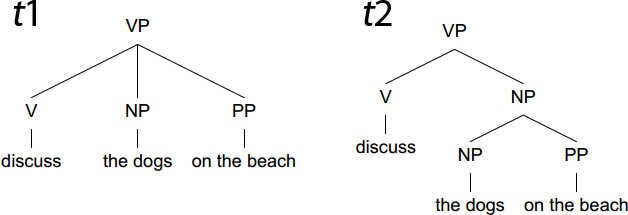
\includegraphics[scale=0.45]{figures/discuss-frame-preference-example.png}
	\caption{Probabilistic Parsing with Frame Preferences to Find Single Preferred Parse of Sentence \textit{"discuss the dogs on the beach"}}
	\label{fig:discuss-frame-probability-example}
\end{figure}

Figure \ref{fig:keep-frame-probability-example} shows two potential parses, $t_1$ and $t_2$ for the sentence \textit{"keep the dogs on the beach"}. Notice how the only difference between this sentence and the last is the verb "keep" (replaces "discuss"). Using the same construction and frame probabilities, the probabilities of each parse are:
\begin{equation}
\begin{aligned}[b]
	P(t_1) = 0.15 \times 0.81 = 0.12 \\
	P(t_2) = 0.19 \times 0.39 \times 0.14 = 0.01 \\
\end{aligned}
\end{equation}
Therefore, the preferred parse is $t_1$. The dogs themselves are being kept on the beach. It is not the dogs that are \textit{currently} on the beach that are being kept by some other party.

\begin{figure}[H]
	\centering
	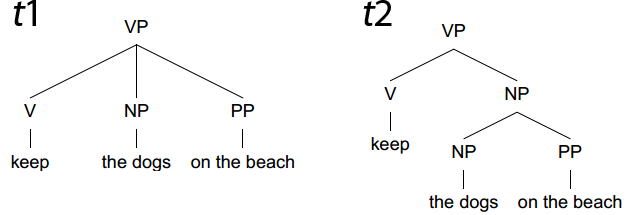
\includegraphics[scale=0.45]{figures/keep-frame-preference-example.png}
	\caption{Probabilistic Parsing with Frame Preferences to Find Single Preferred Parse of Sentence \textit{"keep the dogs on the beach"}}
	\label{fig:keep-frame-probability-example}
\end{figure}

\subsection{Local Ambiguity}

\textbf{Local ambiguity} is when only a \textit{part} of a sentence is ambiguous, and the whole sentence is not. An example:
\begin{quote}
	The old train ... the young. \\
	The old train ... left the station.
\end{quote}
The ambiguous part is "old train". Does this mean a train is old, or whether old people are training something? Local ambiguity makes automatic parsing \textbf{inefficient} , because it means the parser performs a lot of backtracking.

\textbf{Serial parsers} build trees through successive rule selection (e.g. DFS). If more than one rule applies (\textbf{choice point}), one of the rules are chosen based on a selection rule (e.g. "first in first out"). If the resultant tree turns out to be impossible, return to the choice point (\textbf{backtracking}) and reparse from there. 

\paragraph{\textbf{NOTE: }} An example of a selection method for rules is \textbf{local attachment}, which chooses the rule with the most symbols (either terminal or non-terminal).
\paragraph{}

\textbf{Parallel parsers}, like serial parsers, build parse trees through successive rule selection. If more than one rule applies, \textbf{create a new tree for each rule}. All the different trees/possibilities are pursued in \textbf{parallel}. If one of the trees turns out to be impossible, drop it. One issue with parallel parsing is that the number of parse trees can \textbf{grow exponentially}, which means an exponential number of processes are required (not feasible).

\subsubsection{Garden Paths}

A \textbf{garden path} is a sentence where the \textbf{initial part of the sentence is locally ambiguous} and one of the parses of that initial part is preferable to humans (i.e. more likely). However, the dispreferred parse is actually the correct one for the sentence (so the human/parser has to backtrack).

Examples of Garden Paths include:
\begin{quote}
	\textit{"The old man the boats."} \\
	\textit{"Ross baked the cake in the freezer."} \\
	\textit{"The teachers taught by the Berlitz method passed the test."} \\
	\textit{"The complex houses married and single students and their families.."} \\
\end{quote}

If you always only keep one interpretation (the most likely) of a sentence in your mind at a time at a time (i.e. serial parsing), then garden paths will \textit{always} cause you to backtrack. If you always keep every possible interpretation in your mind at the same time (i.e. parallel parsing), then no backtracking is \textit{ever} required. Fully parallelising parsing is not feasible however, so \textbf{bounded parallelism} can be used as a middle ground.

\subsubsection{Jurafsky's Cognitive Model (Parse Tree Pruning)}

\textbf{Jurafsky's probabilistic model} of lexical and syntactic access and disambiguation can be used to consider multiple parses of a sentence in \textbf{parallel}. It:
\begin{itemize}
	\item computes interpretations/parses in parallel
	\item each interpretation is assigned a probability via PCFGs, frame probabilities (techniques already covered here) and Bayesian modelling 
	\item prunes a certain number of unlikely interpretations/trees to \textbf{bound the number of processes running in parallel} and combat memory limitations
\end{itemize}
The fact it bounds the number of parses being considered in parallel makes the model \textbf{computationally feasible} to run even on the most complex of sentences with many, many different parses. This is known as \textbf{bounded parallelism}.

Jurafsky's model makes a crucial assumption: if the relative probability of a tree falls below a certain value, then it will be \textbf{pruned}. We assume a garden path occurs if the \textbf{probability ratio} is higher than 5:1. This ratio is known as the \textbf{beam width}.

Table \ref{tab:beam-width} shows the probability ratio of various garden path sentences. "the complex houses ..." and "the horse raced ... " are considered to be garden path sentences; the likely parses for these are pruned!

\begin{table}
	\centering
	\begin{tabular}{|l|l|}
		\hline
		\textbf{Sentence} & \textbf{Probability Ratio} \\
		\hline
		the complex houses ... & 267:1 \\
		the horse raced ... & 82:1 \\
		\hline
		the warehouse fires ... & 3.8:1 \\
		the bird found ... & 3.7:1 \\
		\hline
	\end{tabular}
	\caption{Probability Ratio of Different Sentences. The first two are considered to be garden path sentences as their probability ratios are higher than the beam width.}
	\label{tab:beam-width}
\end{table}

Open issues issues with the Jurafsky model include:
\begin{itemize}
	\item \textbf{Coverage of Garden Paths} -- Jurafsky used \textbf{hand-crafted} examples of Garden Paths. Can we use a probabilistic parser that is trained on a real corpus to find more garden paths (and new, unseen ones)?
	\item \textbf{Memory Limitations} -- how can the model be augmented to take memory limitations into account more?
	\item \textbf{Crosslinguistics} -- does the model work for languages \textbf{other than English}?
\end{itemize}

\end{document}
